% --- NEW Chapter 3: Mechanical Design and Assembly ---
\chapter{Mechanical Design and Assembly}
\label{chap:mechanical_design_assembly}

\section{Introduction}
\label{sec:mech_intro}
This chapter details the mechanical design and physical construction of the Smart Cleaning Robot prototype. It covers the overall structural design, the \hyperref[term:cad]{CAD}-based development of individual components using SolidWorks, material considerations, and the assembly of the robot's chassis, the encoder-based drive system for precision tracking, and the integrated vacuum cleaning mechanism. The dimensions for the custom-designed parts in SolidWorks were determined based on the physical sizes of the selected electronic and mechanical components. A comprehensive Bill of Materials, including all components and associated costs, can be found in Appendix \ref{app:bom}.
The design prioritizes functionality, ease of assembly for a prototype, and component housing while also considering the challenges encountered during fabrication and iteration.
The overall dimensions of the assembled robot are approximately 35cm in diameter and 17cm in height (excluding the small wheel clearance). The fully assembled prototype has an approximate total weight of 2.65 kg.

\section{Mechanical Components Summary}
The key mechanical components providing the robot's structure and non-powered mobility are summarized in Table~\ref{tab:mechanical_components}. This table focuses only on the structural parts; the full list of electrical components is detailed in Chapter~\ref{chap:electrical_control_performance}, and a comprehensive Bill of Materials for all parts can be found in Appendix \ref{app:bom}.

\begingroup
\small % Make font smaller for the table content
\sloppy % Allow more flexible word spacing
\renewcommand{\arraystretch}{1.2} % Add some vertical padding
\begin{longtable}{|L{4.2cm}|p{2.3cm}|L{2.8cm}|L{3cm}|}
\caption{Mechanical Components List} \label{tab:mechanical_components} \\
\hline
\textbf{Component} & \textbf{Photo} & \textbf{Dimensions (cm)} & \textbf{Material} \\ \hline
\endfirsthead

\multicolumn{4}{c}%
{{\tablename\ \thetable\ -- \textit{Continued from previous page}}} \\
\hline
\textbf{Component} & \textbf{Photo} & \textbf{Dimensions (cm)} & \textbf{Material} \\ \hline
\endhead

\hline
\endlastfoot

% --- START OF MECHANICAL COMPONENTS ---

\textbf{Custom 3D-Printed Chassis} & 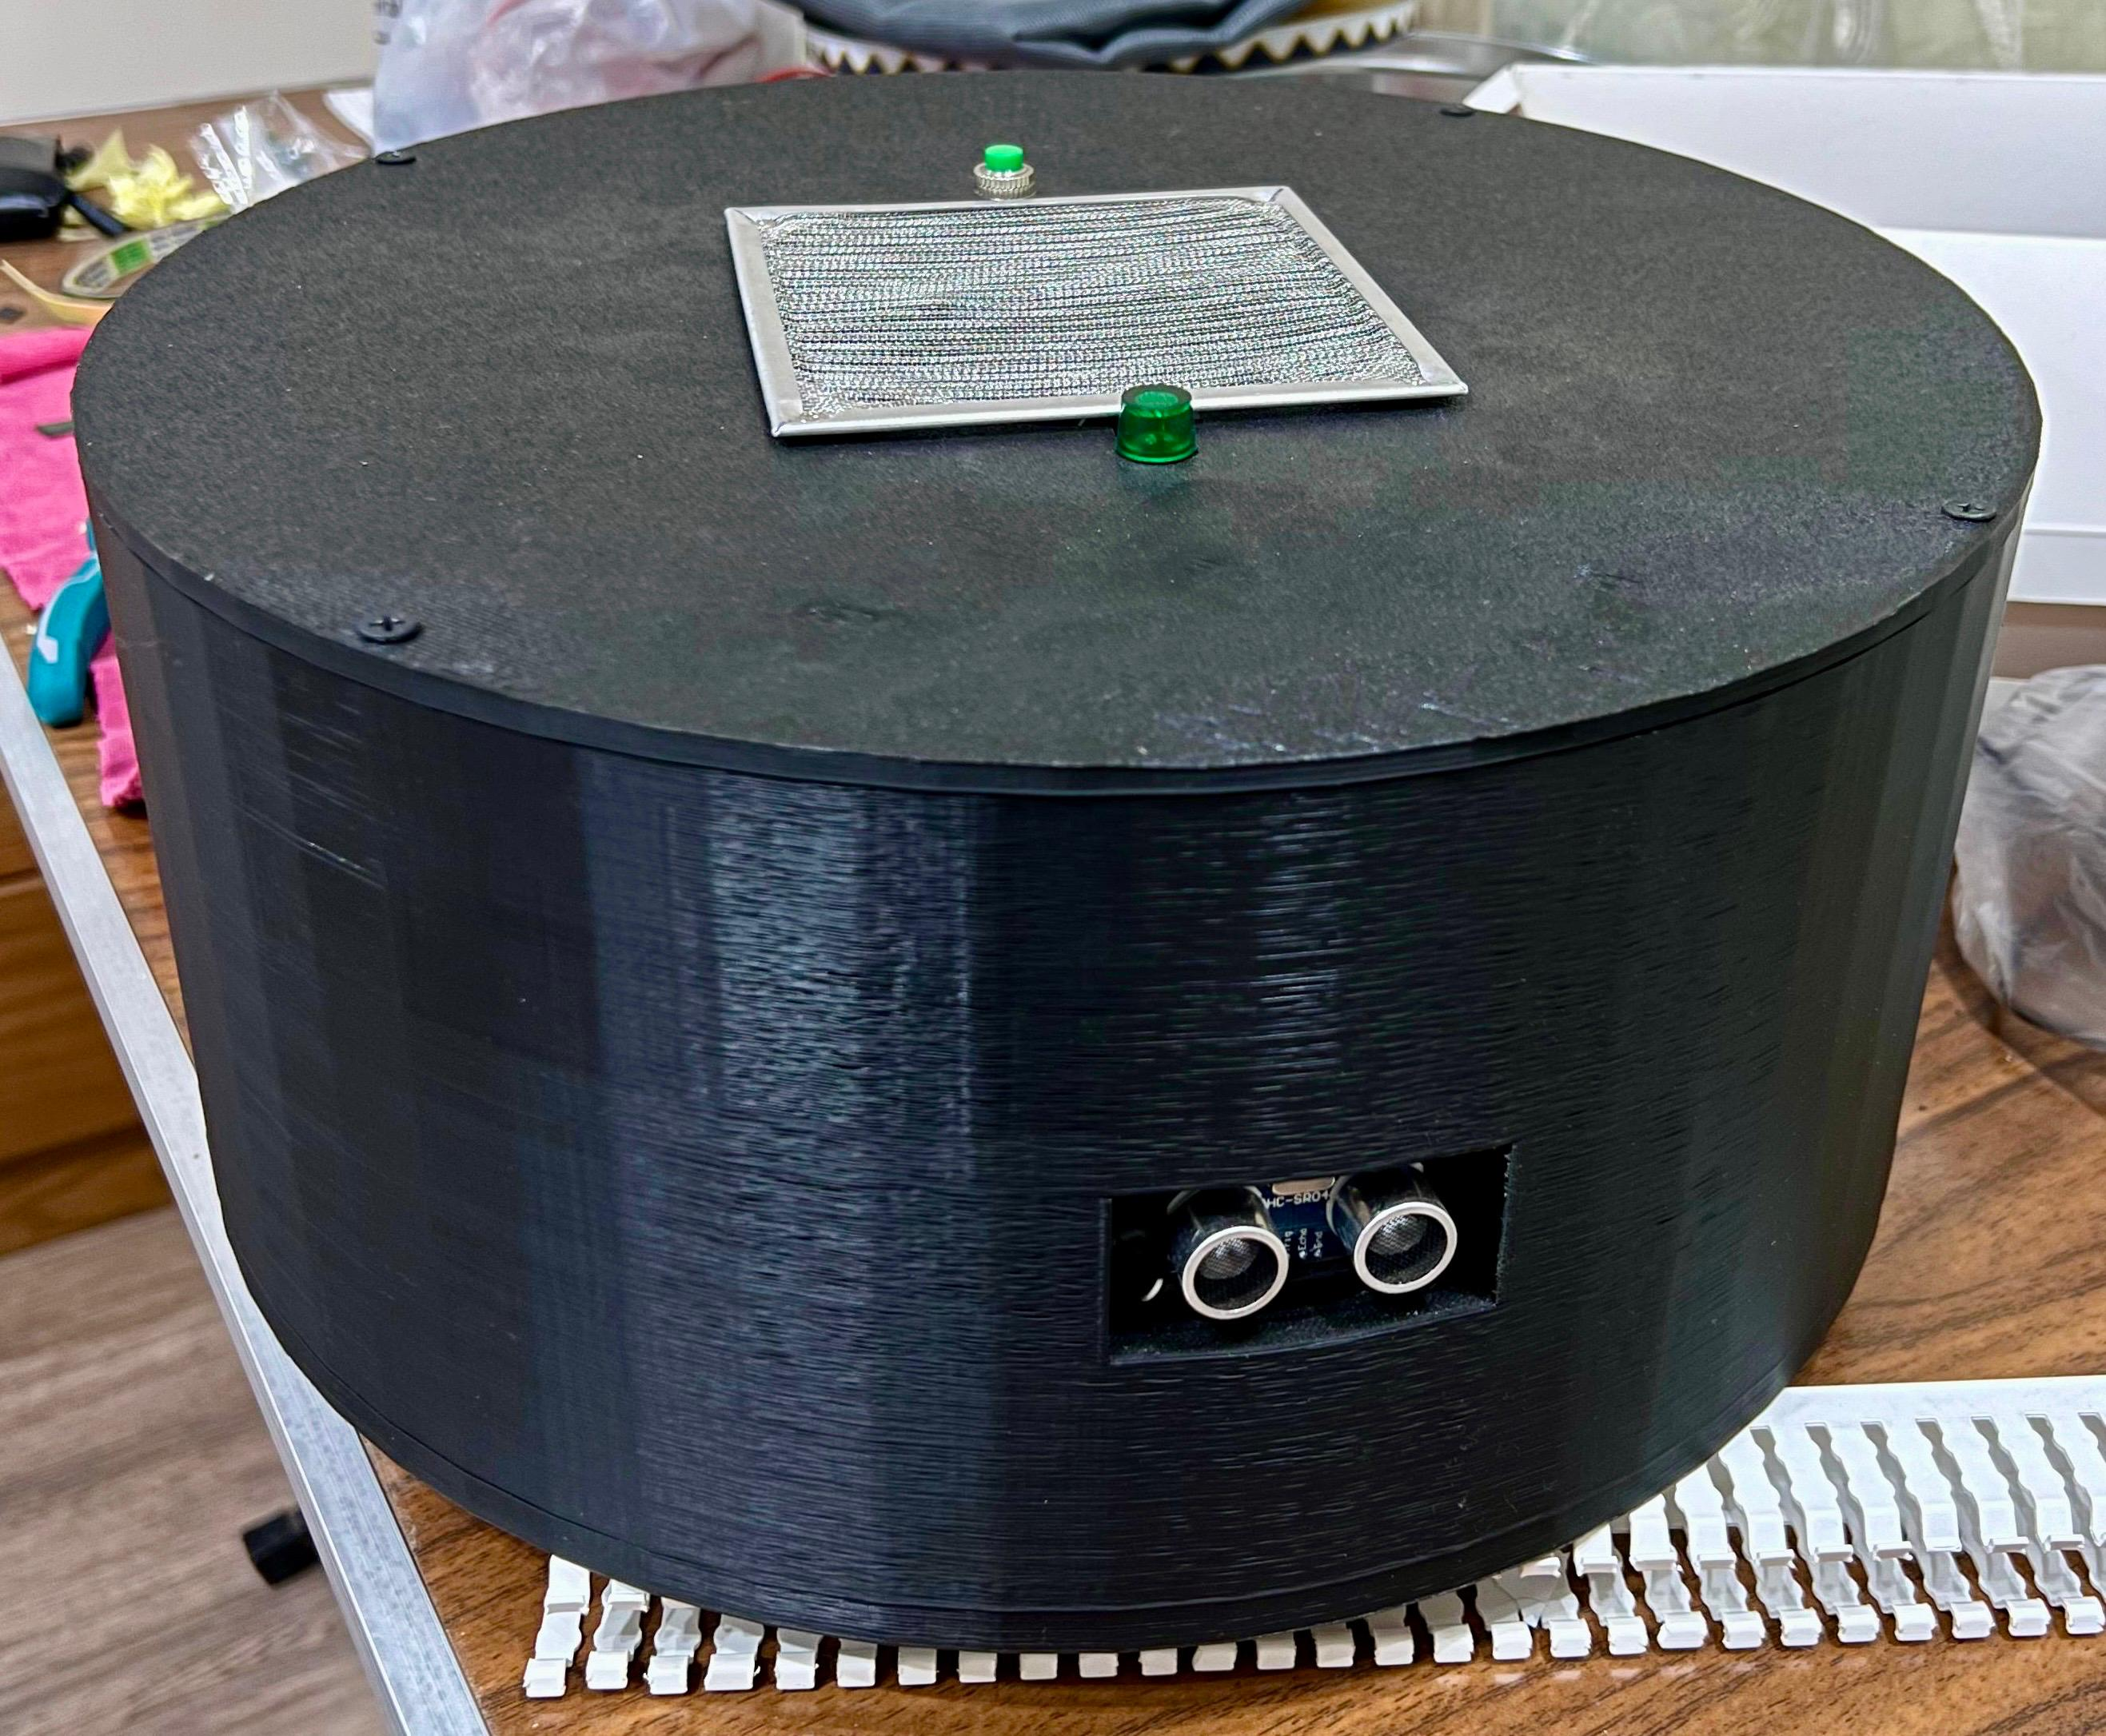
\includegraphics[width=0.9\linewidth, keepaspectratio]{images/photos/robot_assembled_iso.jpg} & $\varnothing \approx 35$, H $\approx 17$ & \hyperref[term:pla]{PLA}+ \\ \hline

\textbf{Custom 3D-Printed Debris Chamber} & 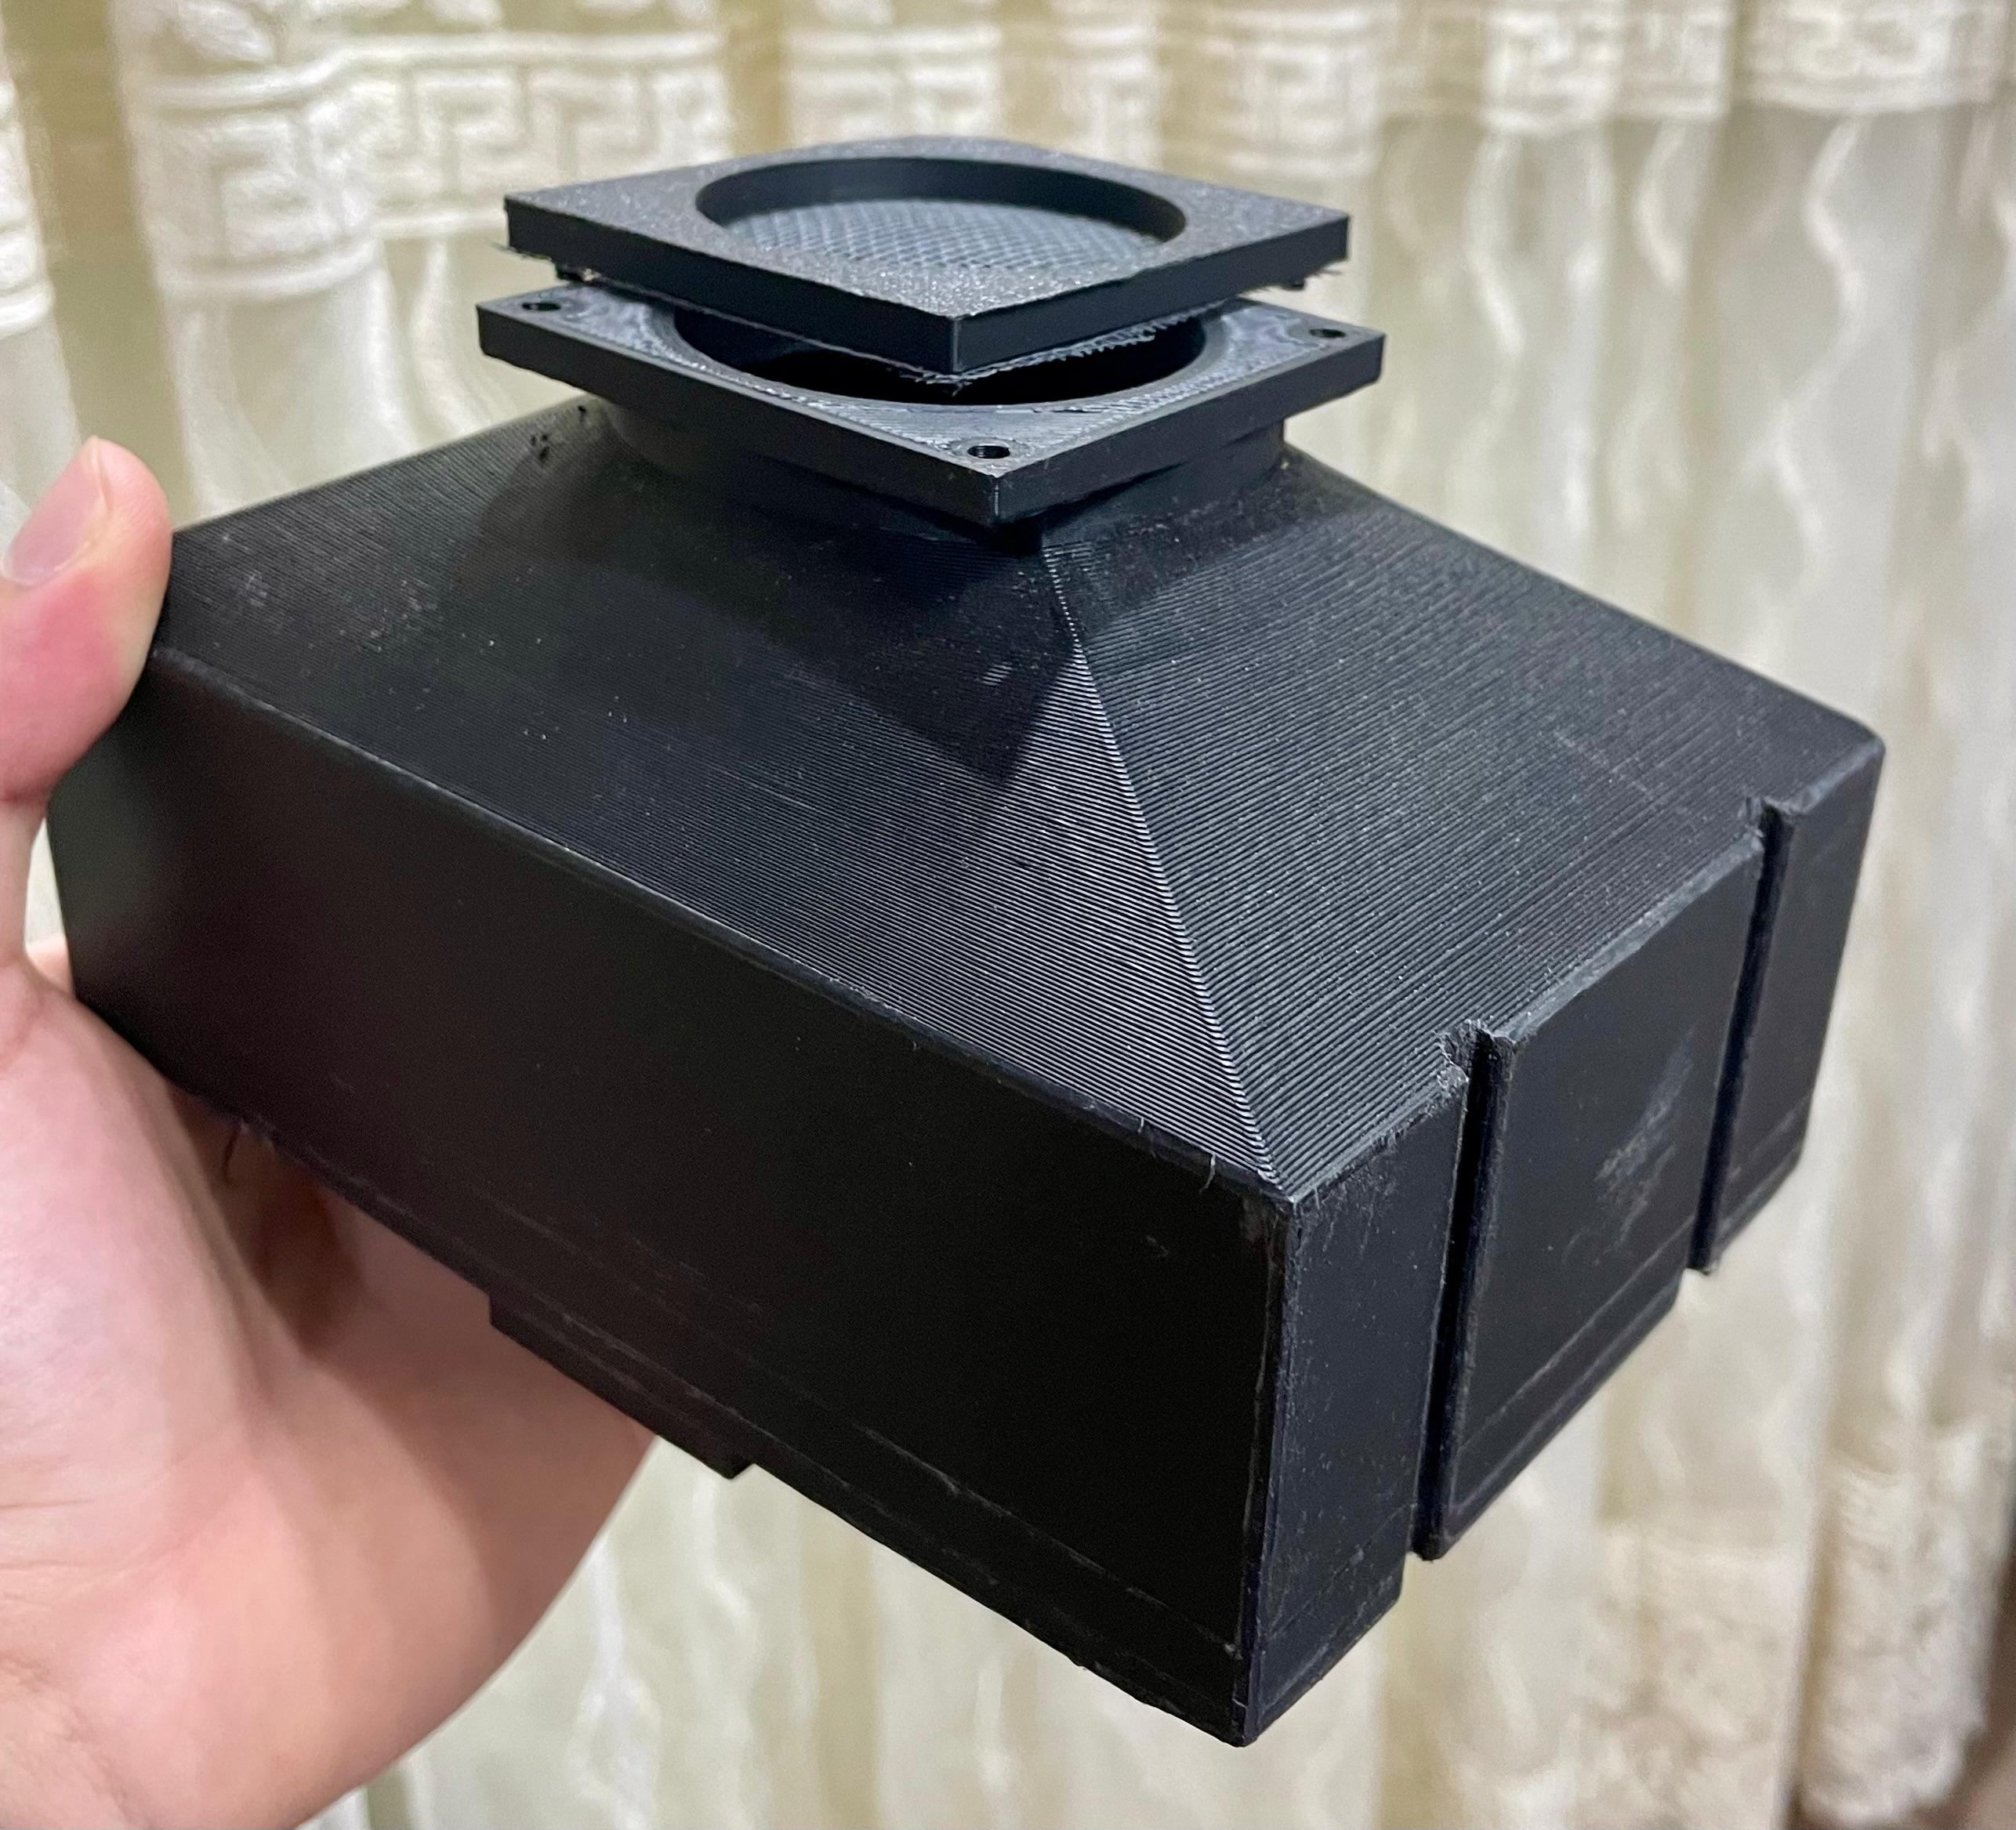
\includegraphics[width=0.9\linewidth, keepaspectratio]{images/photos/debris_chamber_photo.jpg} & WxLxH: 10.5$\times$16$\times$8 & \hyperref[term:pla]{PLA}+ \\ \hline

\href{https://www.maamoon.com/product-page/66mm-robot-smart-car-wheel-tyre}{\textbf{\textcolor{darkblue}{Robot Wheels}}} & 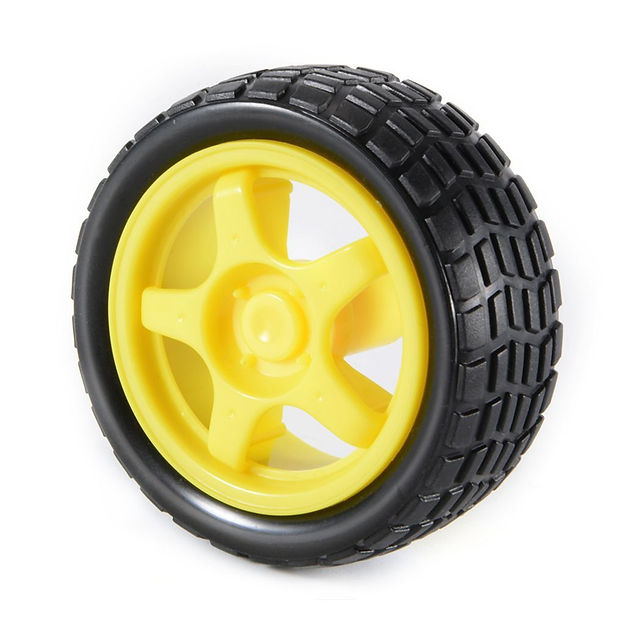
\includegraphics[width=0.9\linewidth, keepaspectratio]{images/components/wheel_66mm.jpg} & $\varnothing$: 6.6, W: 2.8 & Plastic Rim, Rubber Tyre \\ \hline

\href{https://www.ram-e-shop.com/shop/ro-wheel-caster-small-metal-caster-wheel-20-mm-robot-wheel-max-load-15kg-7010}{\textbf{\textcolor{darkblue}{Metal Caster Wheel}}} & 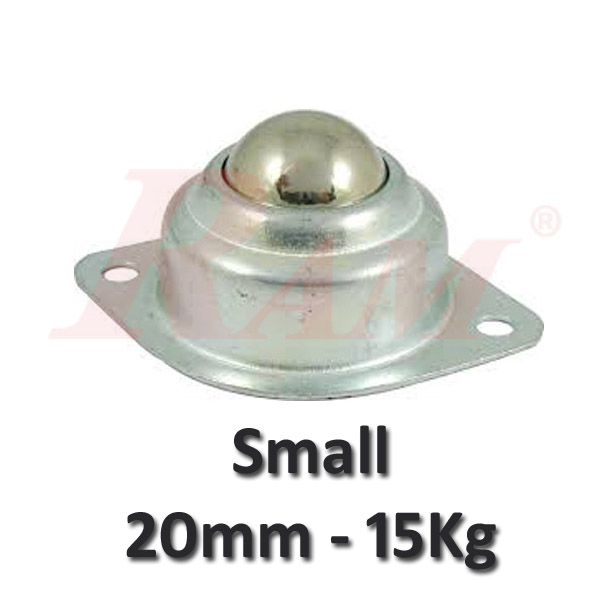
\includegraphics[width=0.9\linewidth, keepaspectratio]{images/components/caster_wheel.jpg} & Height: 2.0, Wheel $\varnothing$: 1.5 & Steel Body and Ball \\ \hline

\href{https://www.ram-e-shop.com/shop/spacer-screw-20mm-plastic-screw-shape-snap-in-rivet-pcb-spacer-20mm-5739}{\textbf{\textcolor{darkblue}{PCB Spacers (Snap-in Rivet)}}} & 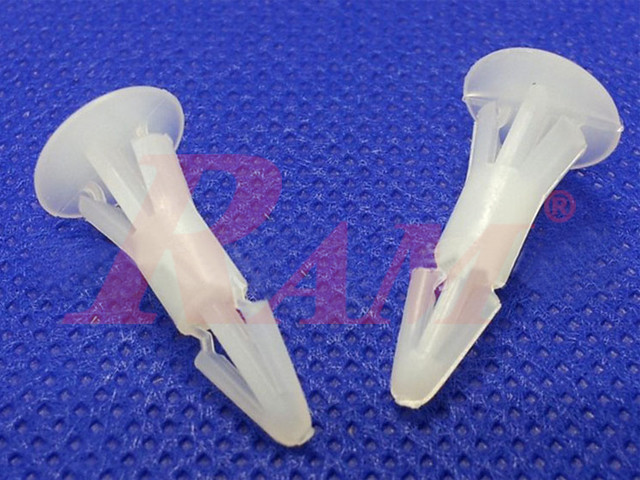
\includegraphics[width=0.9\linewidth, keepaspectratio]{images/components/pcb_spacer.jpg} & Length: 2.0 & Nylon \\ \hline

\href{https://www.ram-e-shop.com/shop/nail-3x05mm-bolt-m3x06-mm-100-screws-bag-6545}{\textbf{\textcolor{darkblue}{Bolts and Nuts (M3)}}} & 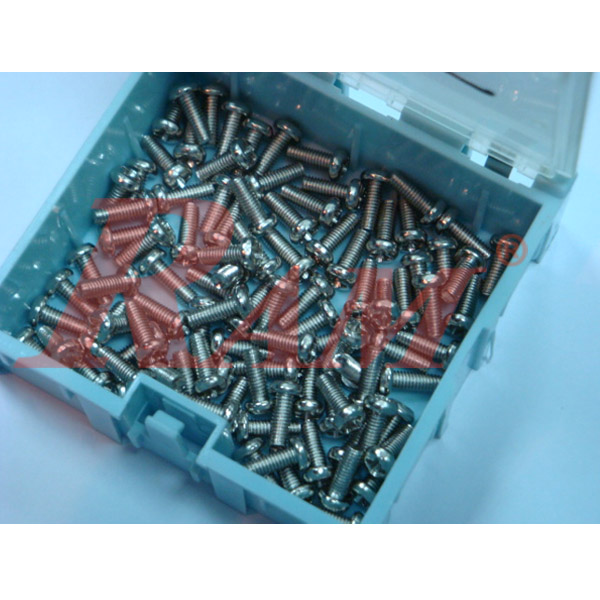
\includegraphics[width=0.9\linewidth, keepaspectratio]{images/components/bolts_m3.jpg} & M3 (various lengths) & Steel \\ \hline

\end{longtable}
\endgroup

\section{Detailed Mechanical Design}
\label{sec:detailed_mechanical_design}

\subsection{Chassis: Structure and Material}
\label{subsec:chassis_structure_material}
The main chassis forms the backbone of the robot, providing mounting points for all components and defining the robot's overall form factor.
The robot features a generally circular chassis, a common design choice for cleaning robots as it aids in maneuverability and helps the robot glance off obstacles rather than getting caught on corners, facilitating navigation in typical household environments.
The custom components were fabricated using \hyperref[term:pla]{PLA}+ filament via an \hyperref[term:fdm]{FDM} 3D printing service; PLA+ was the material offered by the service and is suitable for prototypes due to its ease of printing and adequate strength. Its rigidity is beneficial for creating a stable chassis that prevents flex, ensuring consistent alignment for the drive system and sensors. A substantial wall thickness of approximately 1 cm was utilized for the main structural components to ensure robustness and resistance to impacts during operation.
(Refer to Figure~\ref{fig:solidworks_chassis_views_combined} for detailed CAD views).

\begin{figure}[htbp]
    \centering
    \begin{subfigure}[b]{0.496\textwidth}
        \centering
        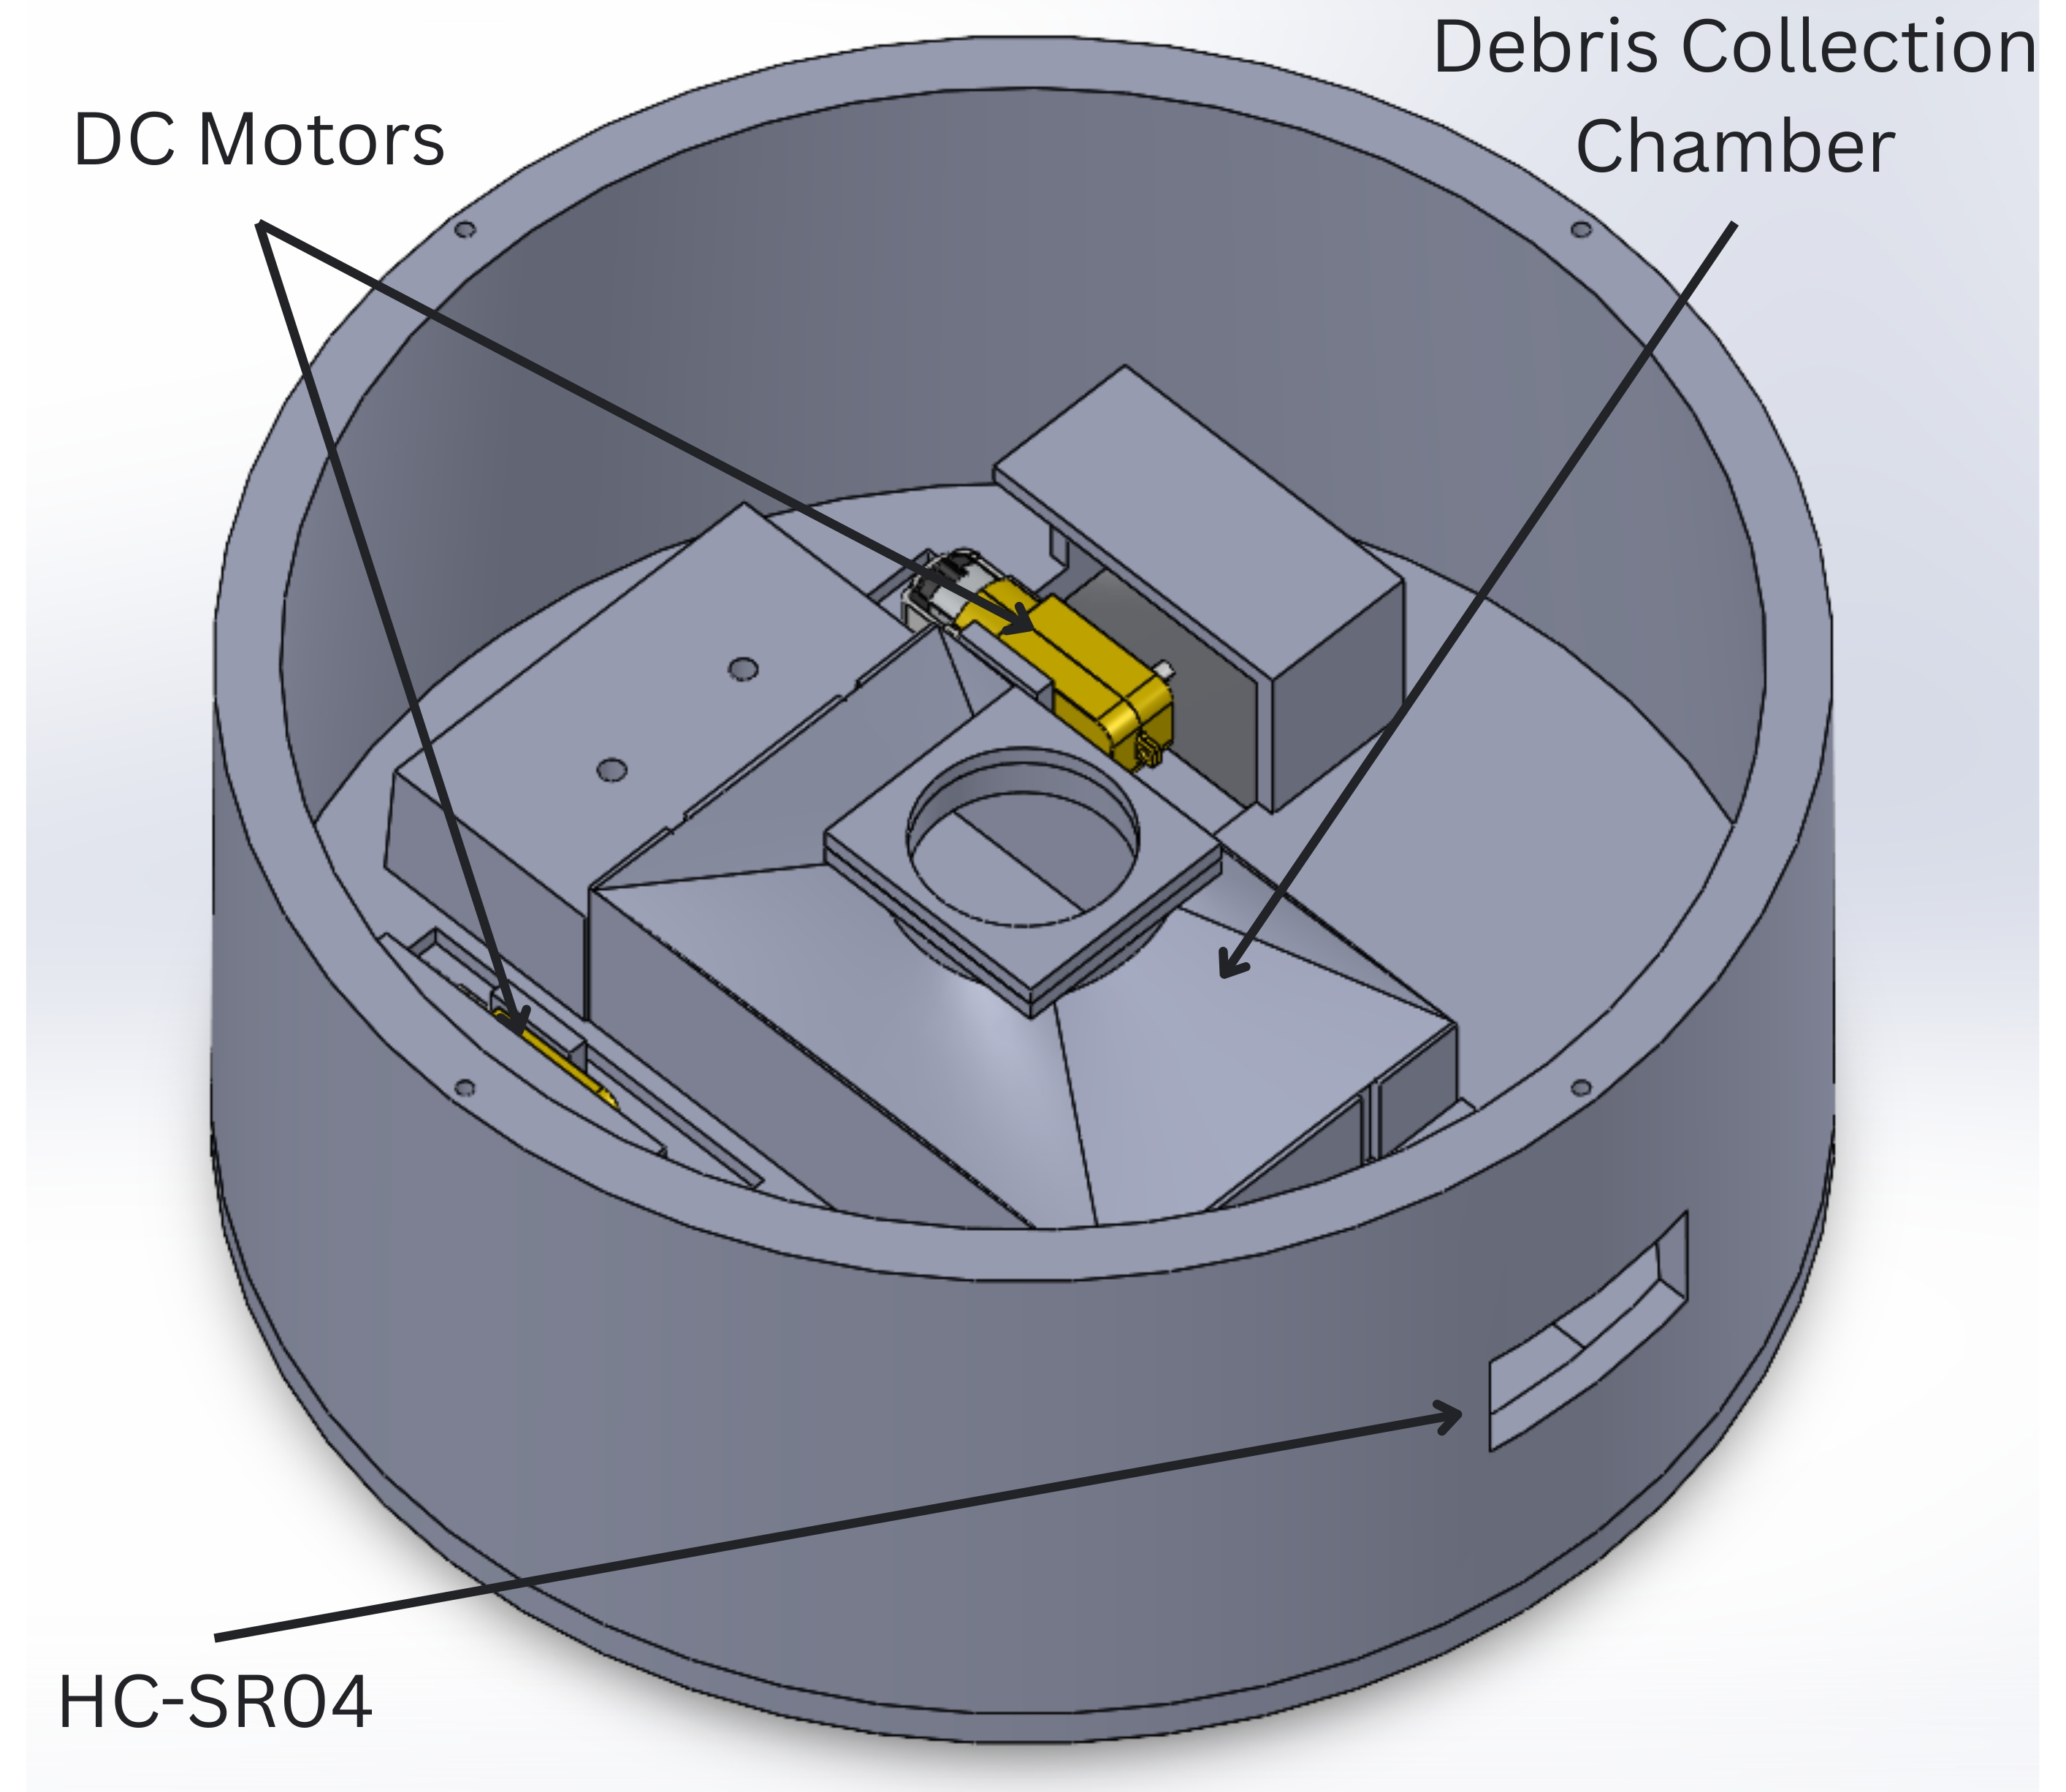
\includegraphics[width=\linewidth, keepaspectratio]{images/cad/chassis_open_isometric.jpg}
        \caption{Isometric view of the open chassis.}
        \label{fig:sw_chassis_iso_open}
    \end{subfigure}
    \hfill
    \begin{subfigure}[b]{0.496\textwidth}
        \centering
        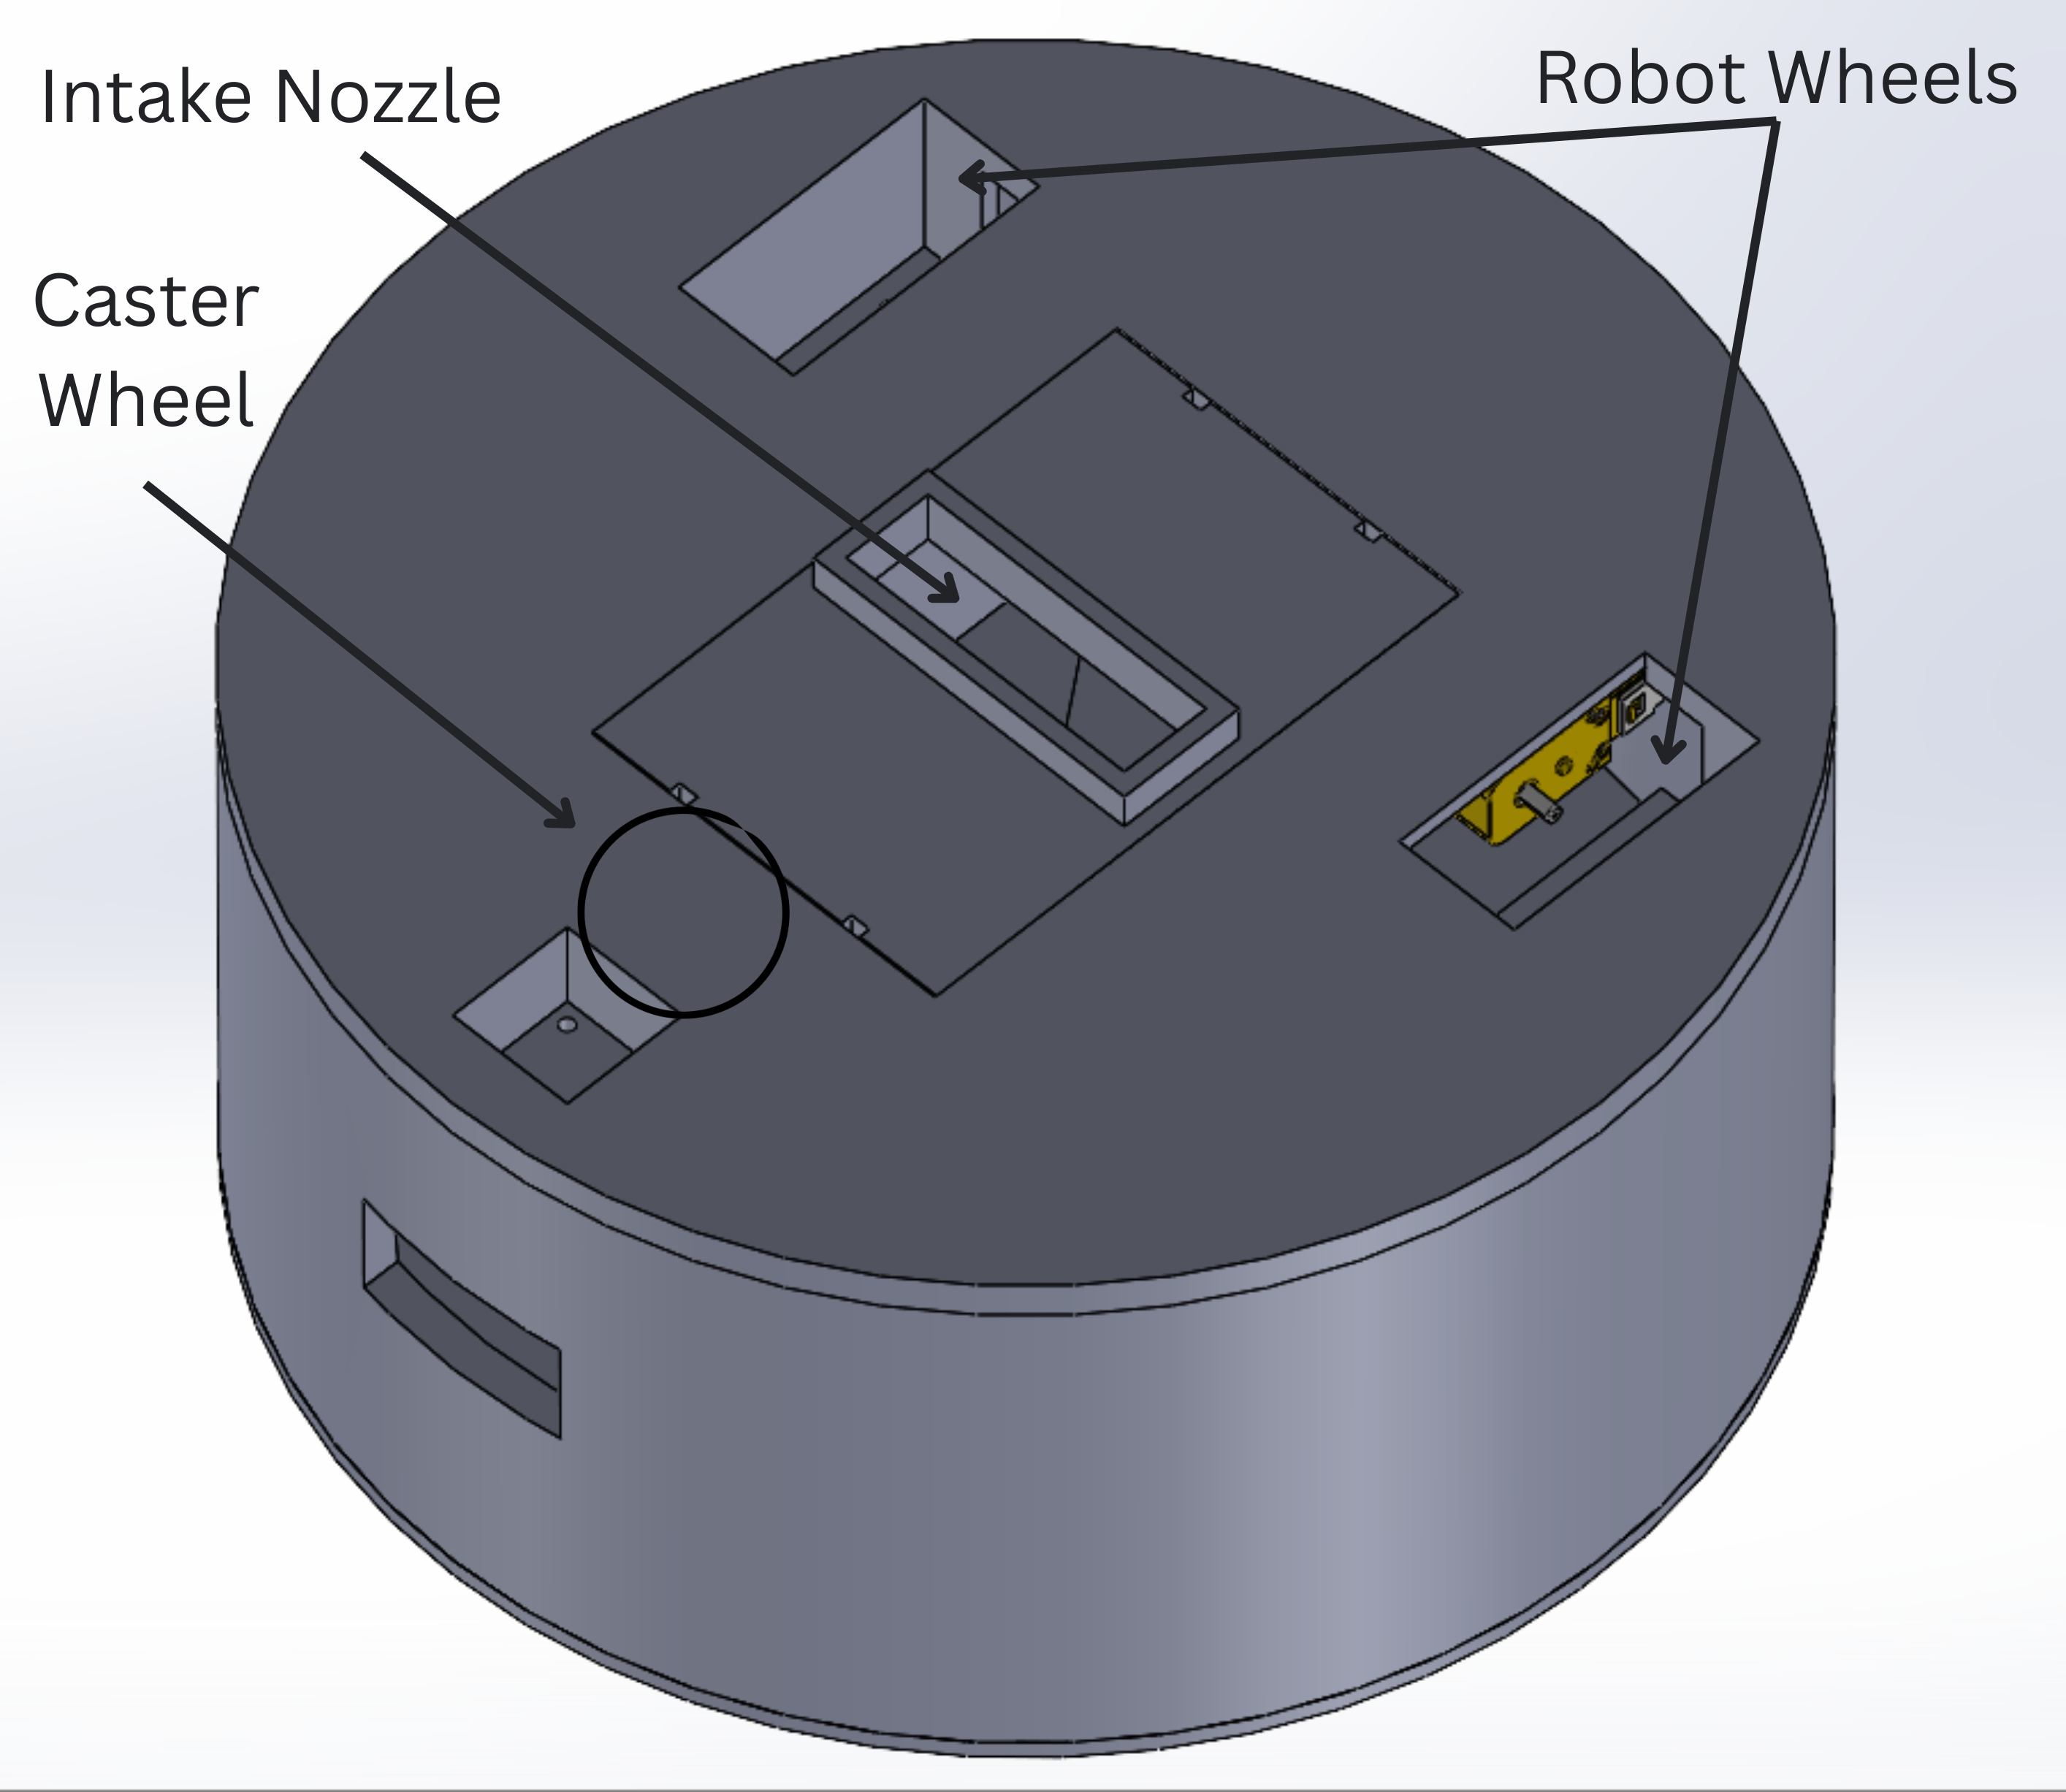
\includegraphics[width=\linewidth, keepaspectratio]{images/cad/chassis_bottom_view.jpg}
        \caption{Bottom CAD view of the chassis.}
        \label{fig:sw_chassis_bottom_cad}
    \end{subfigure}

    \vspace{10pt} % Adds a bit of vertical space between rows of subfigures

    \begin{subfigure}[b]{0.496\textwidth}
        \centering
        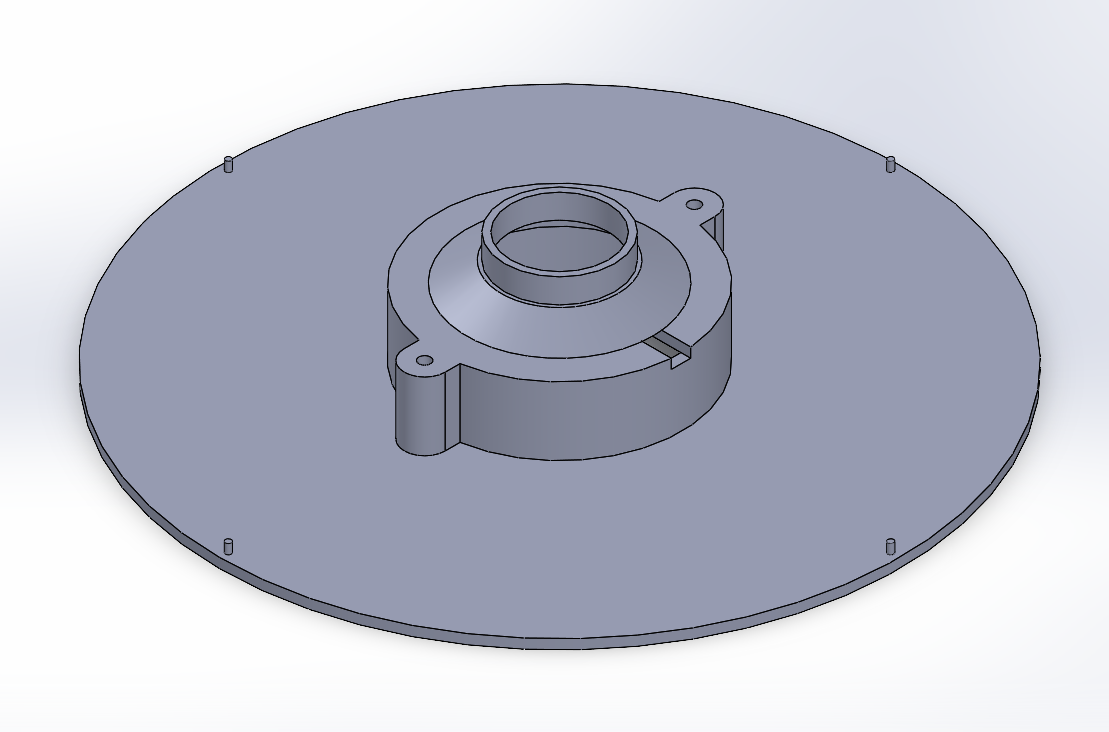
\includegraphics[width=\linewidth, keepaspectratio]{images/cad/chassis_lid_isometric.png}
        \caption{Isometric view of the main robot lid.}
        \label{fig:sw_chassis_lid_iso}
    \end{subfigure}
    \hfill
    \begin{subfigure}[b]{0.496\textwidth}
        \centering
        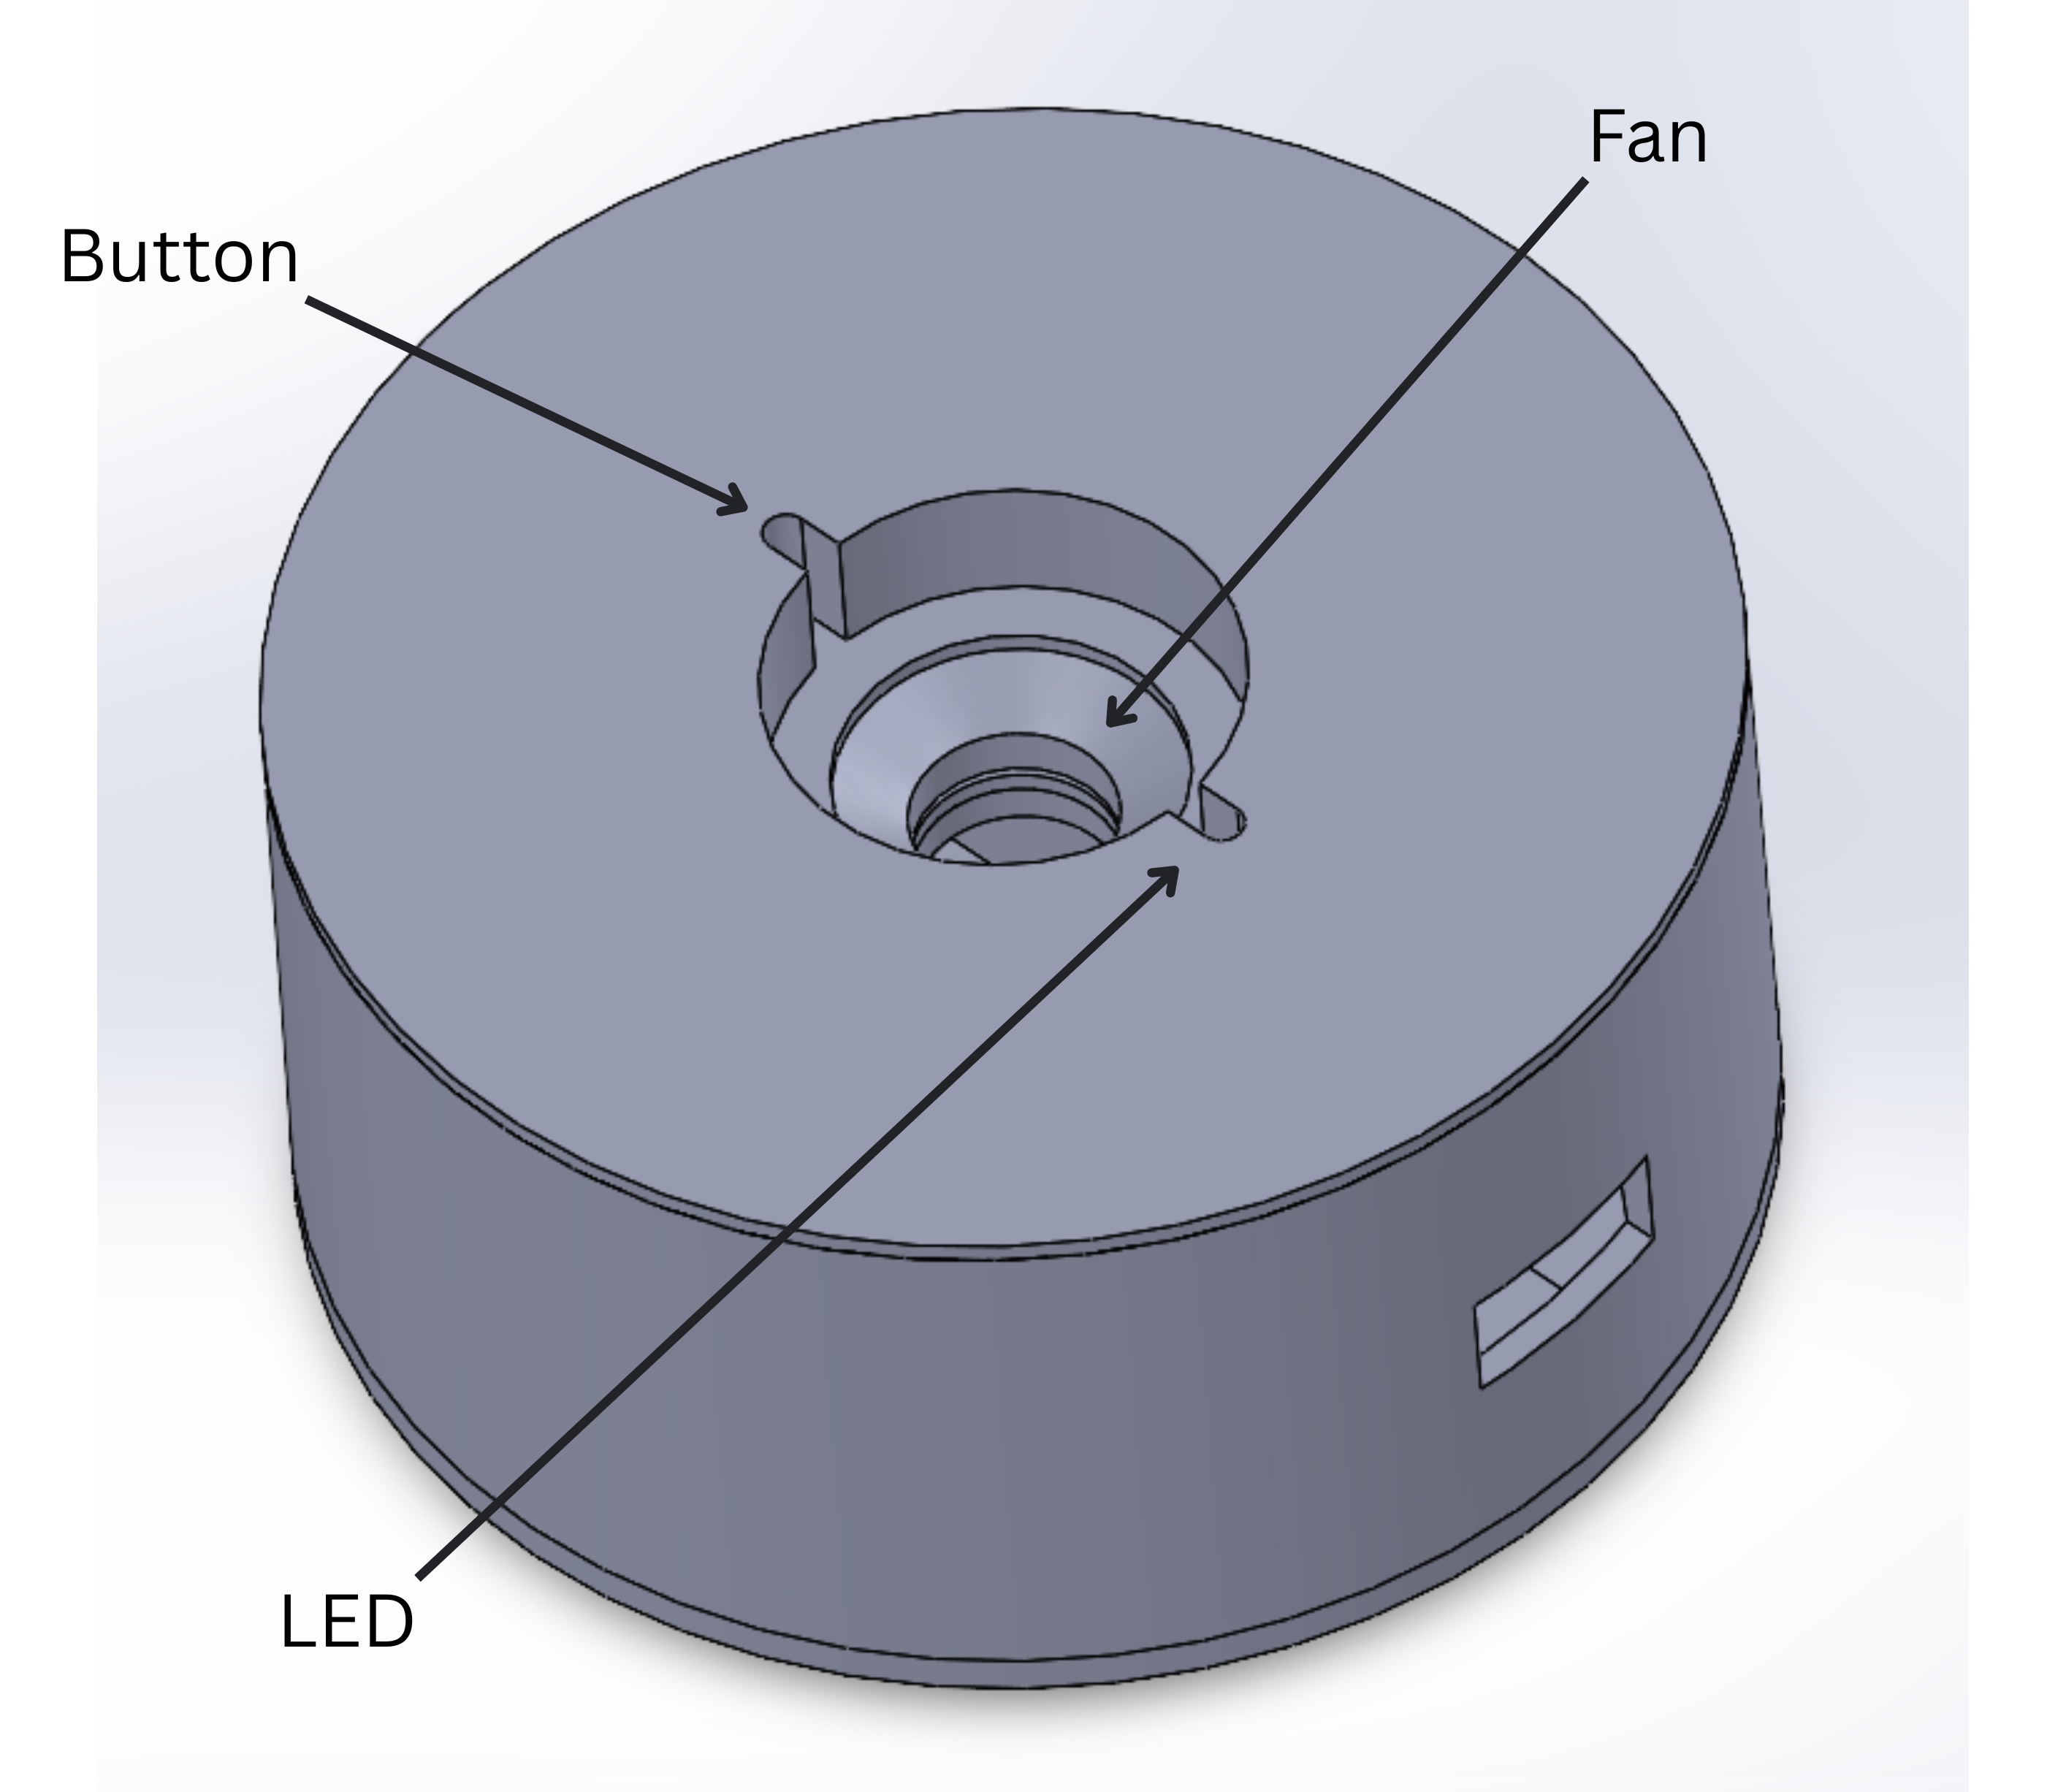
\includegraphics[width=\linewidth, keepaspectratio]{images/cad/chassis_assembled_isometric.jpg}
        \caption{Fully assembled robot isometric view.}
        \label{fig:sw_chassis_iso_closed}
    \end{subfigure}
    \caption{SolidWorks \hyperref[term:cad]{CAD} models illustrating the Smart Cleaning Robot's chassis and assembled form, with annotations to highlight key features.}
    \label{fig:solidworks_chassis_views_combined}
\end{figure}
The chassis is a custom design modeled in SolidWorks and 3D printed. It features:
\begin{itemize}
    \item \textbf{Base Plate}: Provides the primary mounting surface for motors, the caster wheel, and the Debris Collection Chamber. (See Figure~\ref{fig:sw_chassis_bottom_cad} and \ref{fig:sw_chassis_iso_open}). The 12V \hyperref[term:liion]{Li-ion} battery pack is secured between one of the debris chamber's guide blocks (discussed later) and a chassis wall, positioned towards the rear above the drive wheels to enhance traction.
    \item \textbf{Wheel Housings and Motor Mounting Points}: Located at the rear of the chassis, dedicated structures provide partial housing for the wheels. The two \hyperref[term:dc]{DC} gear motors are screwed into small, integrated walls on the chassis; these walls incorporate precise mounting holes and provide lateral support and alignment for the motors. (Visible in Figure~\ref{fig:sw_chassis_iso_open}). These structures were also designed to provide stable mounting points for the IR photoelectric sensors, ensuring the encoder discs that rotate with the wheels pass correctly through their sensing grooves.
    \item \textbf{Sensor Cutout and Mounting}: A dedicated cutout at the front of the chassis houses the \hyperref[term:hcsr04]{HC-SR04}  sensor. A custom bracket was designed to securely hold the sensor within this cutout, ensuring correct alignment for obstacle detection. (Visible in Figure~\ref{fig:sw_chassis_iso_open} and \ref{fig:sw_chassis_iso_closed}).
    \item \textbf{Front Caster Wheel Mount}: The front bottom section of the chassis includes a mounting point for the caster wheel. Due to the unavailability of the initially planned component, an alternative caster wheel was utilized, necessitating an adapted screw mounting method on the chassis base. (See Figure~\ref{fig:sw_chassis_bottom_cad} and Figure~\ref{fig:assembled_robot_bottom_photo}).
    \item \textbf{Central Cutout}: A large central cutout accommodates the Debris Collection Chamber. (Visible in Figure~\ref{fig:sw_chassis_bottom_cad}).
    \item \textbf{Electronics Mounting}: The custom \hyperref[term:pcb]{PCB} (which hosts the Raspberry Pi Pico W, LM2596S buck converter, and sensor voltage divider resistors) and the \hyperref[term:l298n]{L298N} H-bridge motor driver module are elevated from the chassis base using 20mm nylon snap-in rivet PCB spacers. This provides clearance for wiring and protection for the electronics.
\end{itemize}
\begin{figure}[htbp]
    \centering
    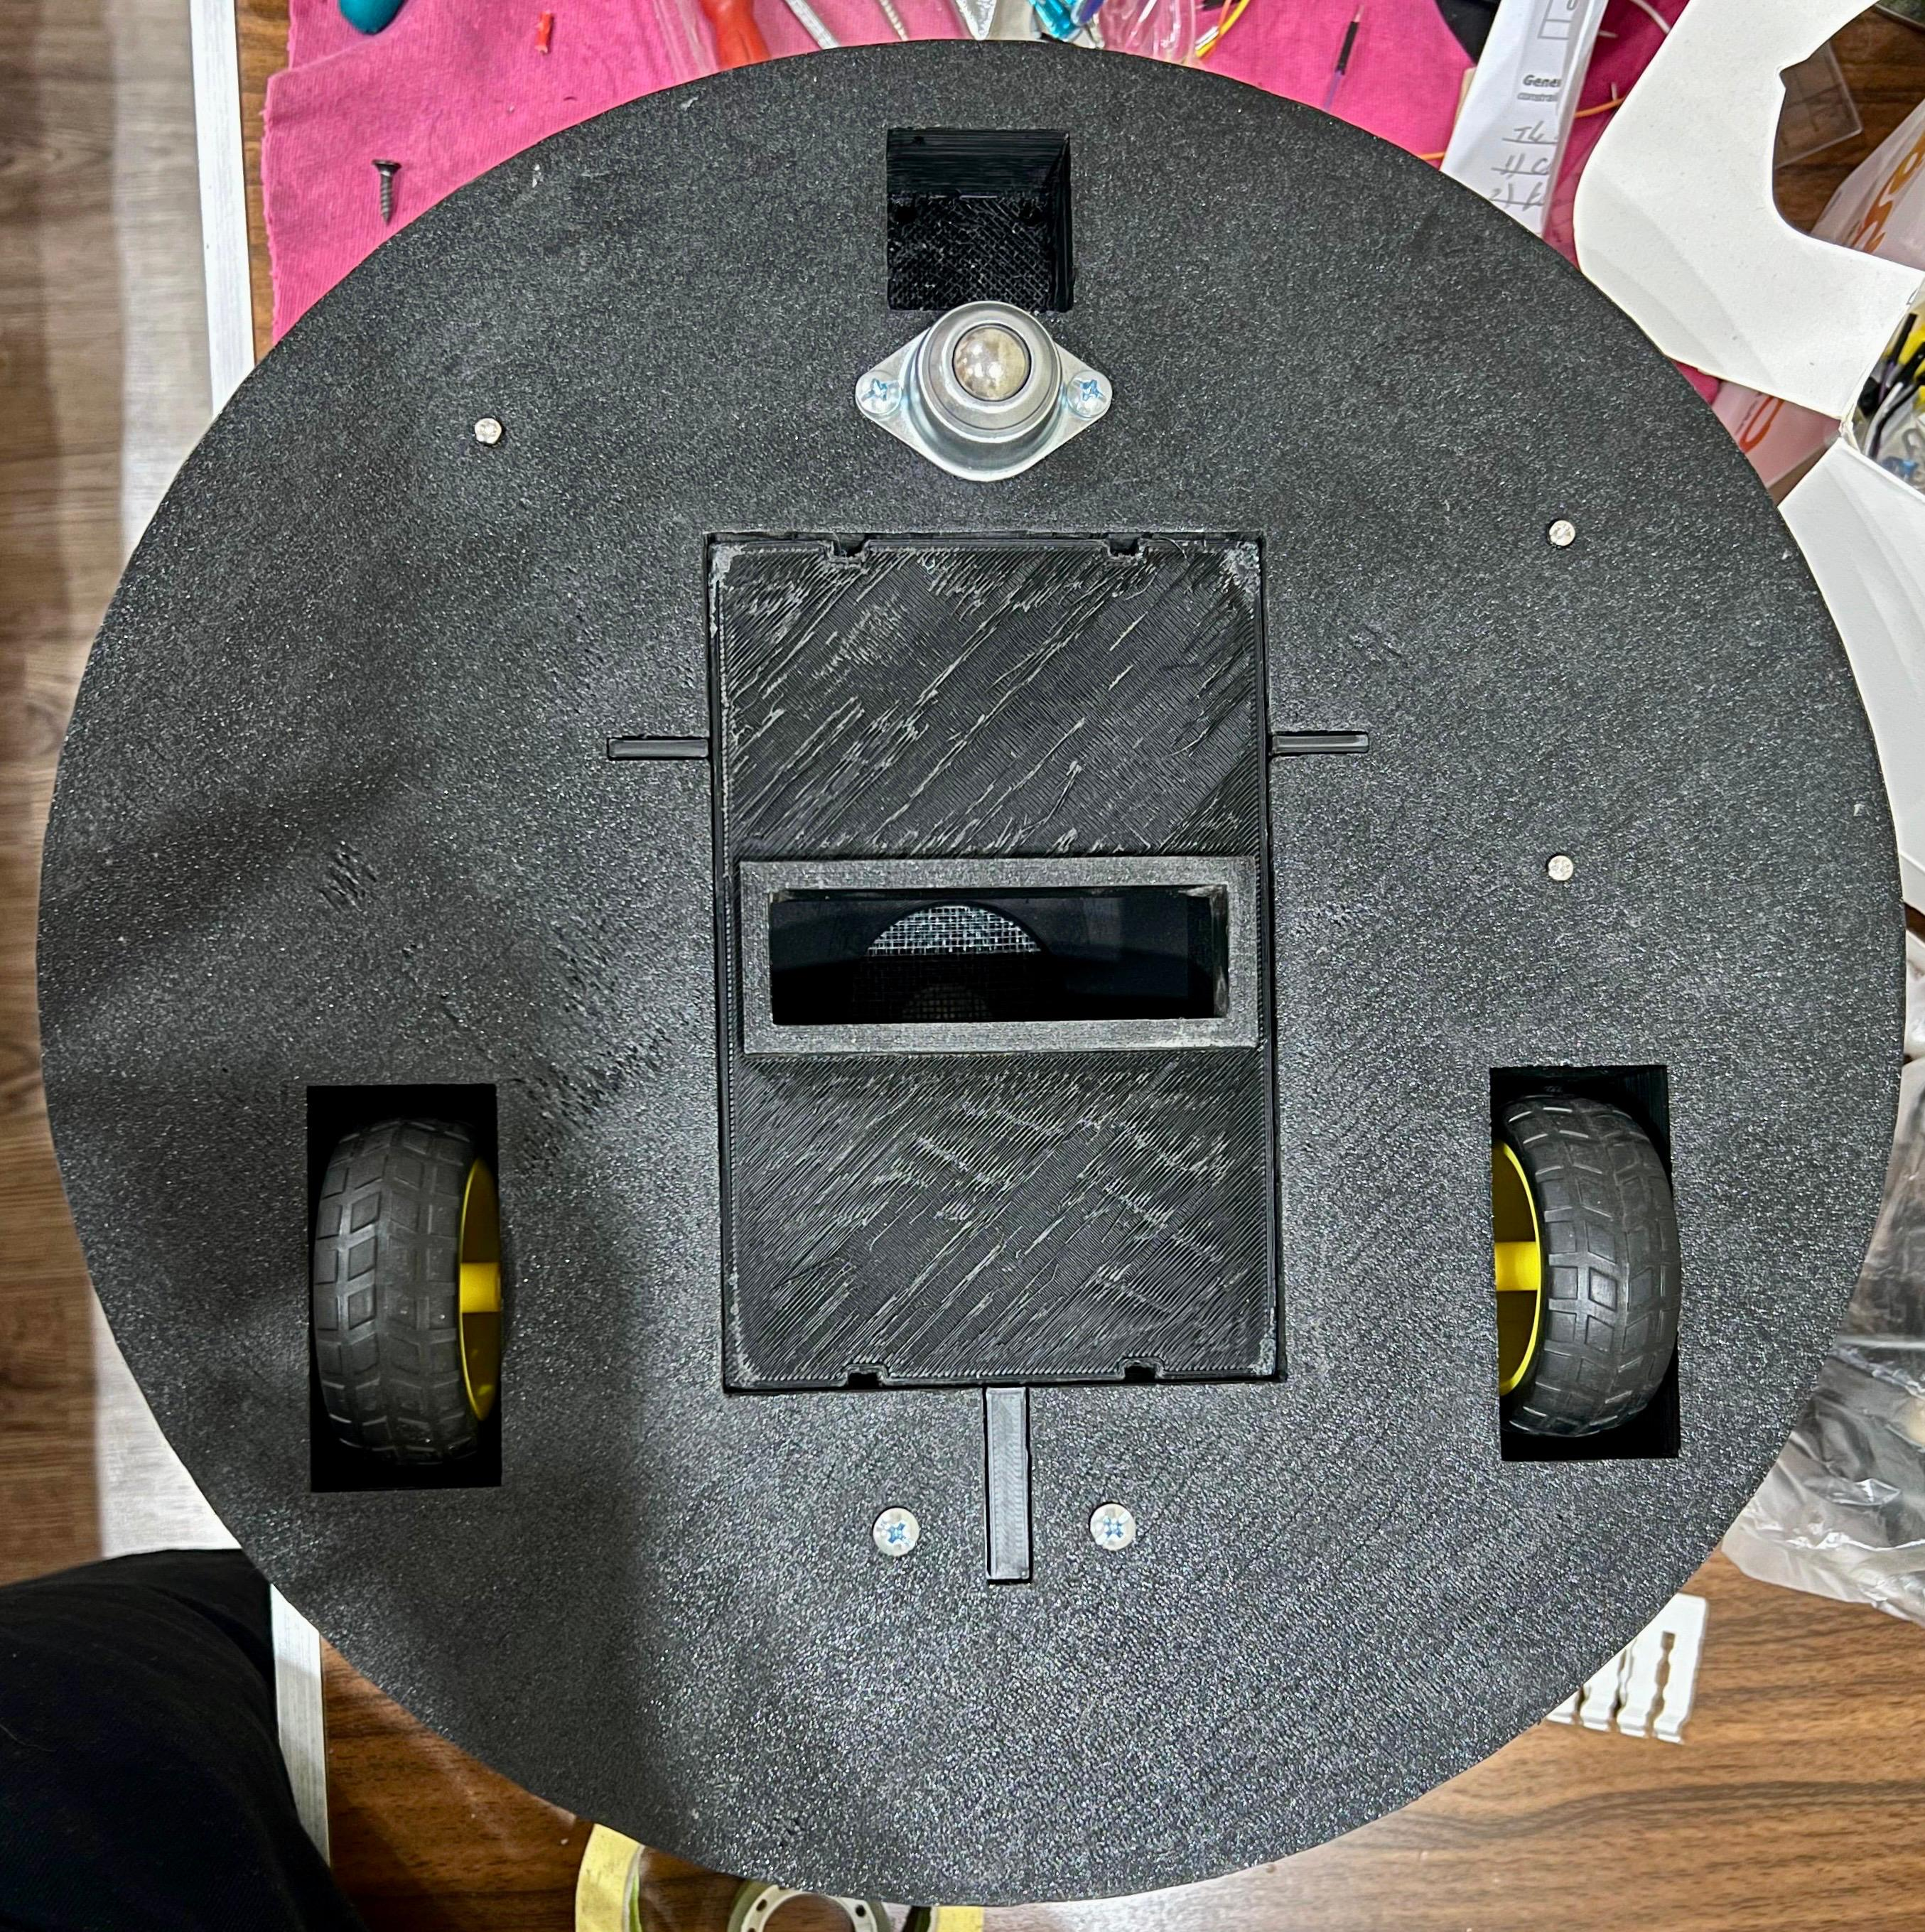
\includegraphics[width=0.75\textwidth, keepaspectratio]{images/photos/robot_bottom_photo.jpg}
    \caption{Bottom view photograph of the assembled Smart Cleaning Robot, showing the caster wheel, drive wheels, and vacuum intake nozzle.}
    \label{fig:assembled_robot_bottom_photo}
\end{figure}


\subsection{Vacuum System Design}
\label{subsec:vacuum_system_design_detailed}
The Debris Collection Chamber is a key sub-assembly designed to collect vacuumed particles. The chamber was designed for a tight clearance fit within the chassis bay to ensure stability and prevent rattling. (See Figure~\ref{fig:solidworks_debris_chamber} for its CAD design and Figure~\ref{fig:debris_chamber_photo} for a photo of the 3D printed part).
\begin{itemize}
    \item \textbf{Chamber Design}: The chamber itself is a custom 3D-printed component. It features a rectangular box base measuring 10.5\,cm in width, 16\,cm in length, and 5.5\,cm in height. From this base, the chamber transitions through a pyramid-like section for an additional 2.5\,cm in height, culminating in a circular outlet of 5\,cm in diameter. This outlet is designed to interface with the vacuum fan and also seats the air filter. The debris inlet, located at the bottom of the chamber, has dimensions of 8.5\,cm x 2.5\,cm.
    \item \textbf{Mounting and Guides}: The method for positioning the chamber within the chassis was refined during development (detailed in Section~\ref{sec:mechanical_assembly_implementation_new}). The final design uses two robust 3D-printed blocks screwed to the chassis base, incorporating guide elements for secure and precise placement.
    \item \textbf{Filter and Lid}: A removable lid is designed for the top of the Debris Collection Chamber to hold an air filter. This lid fits into corresponding features on the chamber for easy removal and a secure fit. The main robot chassis lid (Figure~\ref{fig:sw_chassis_lid_iso}), when closed, presses down on this filter lid, keeping it secure.
\end{itemize}

\begin{figure}[htbp]
    \centering
    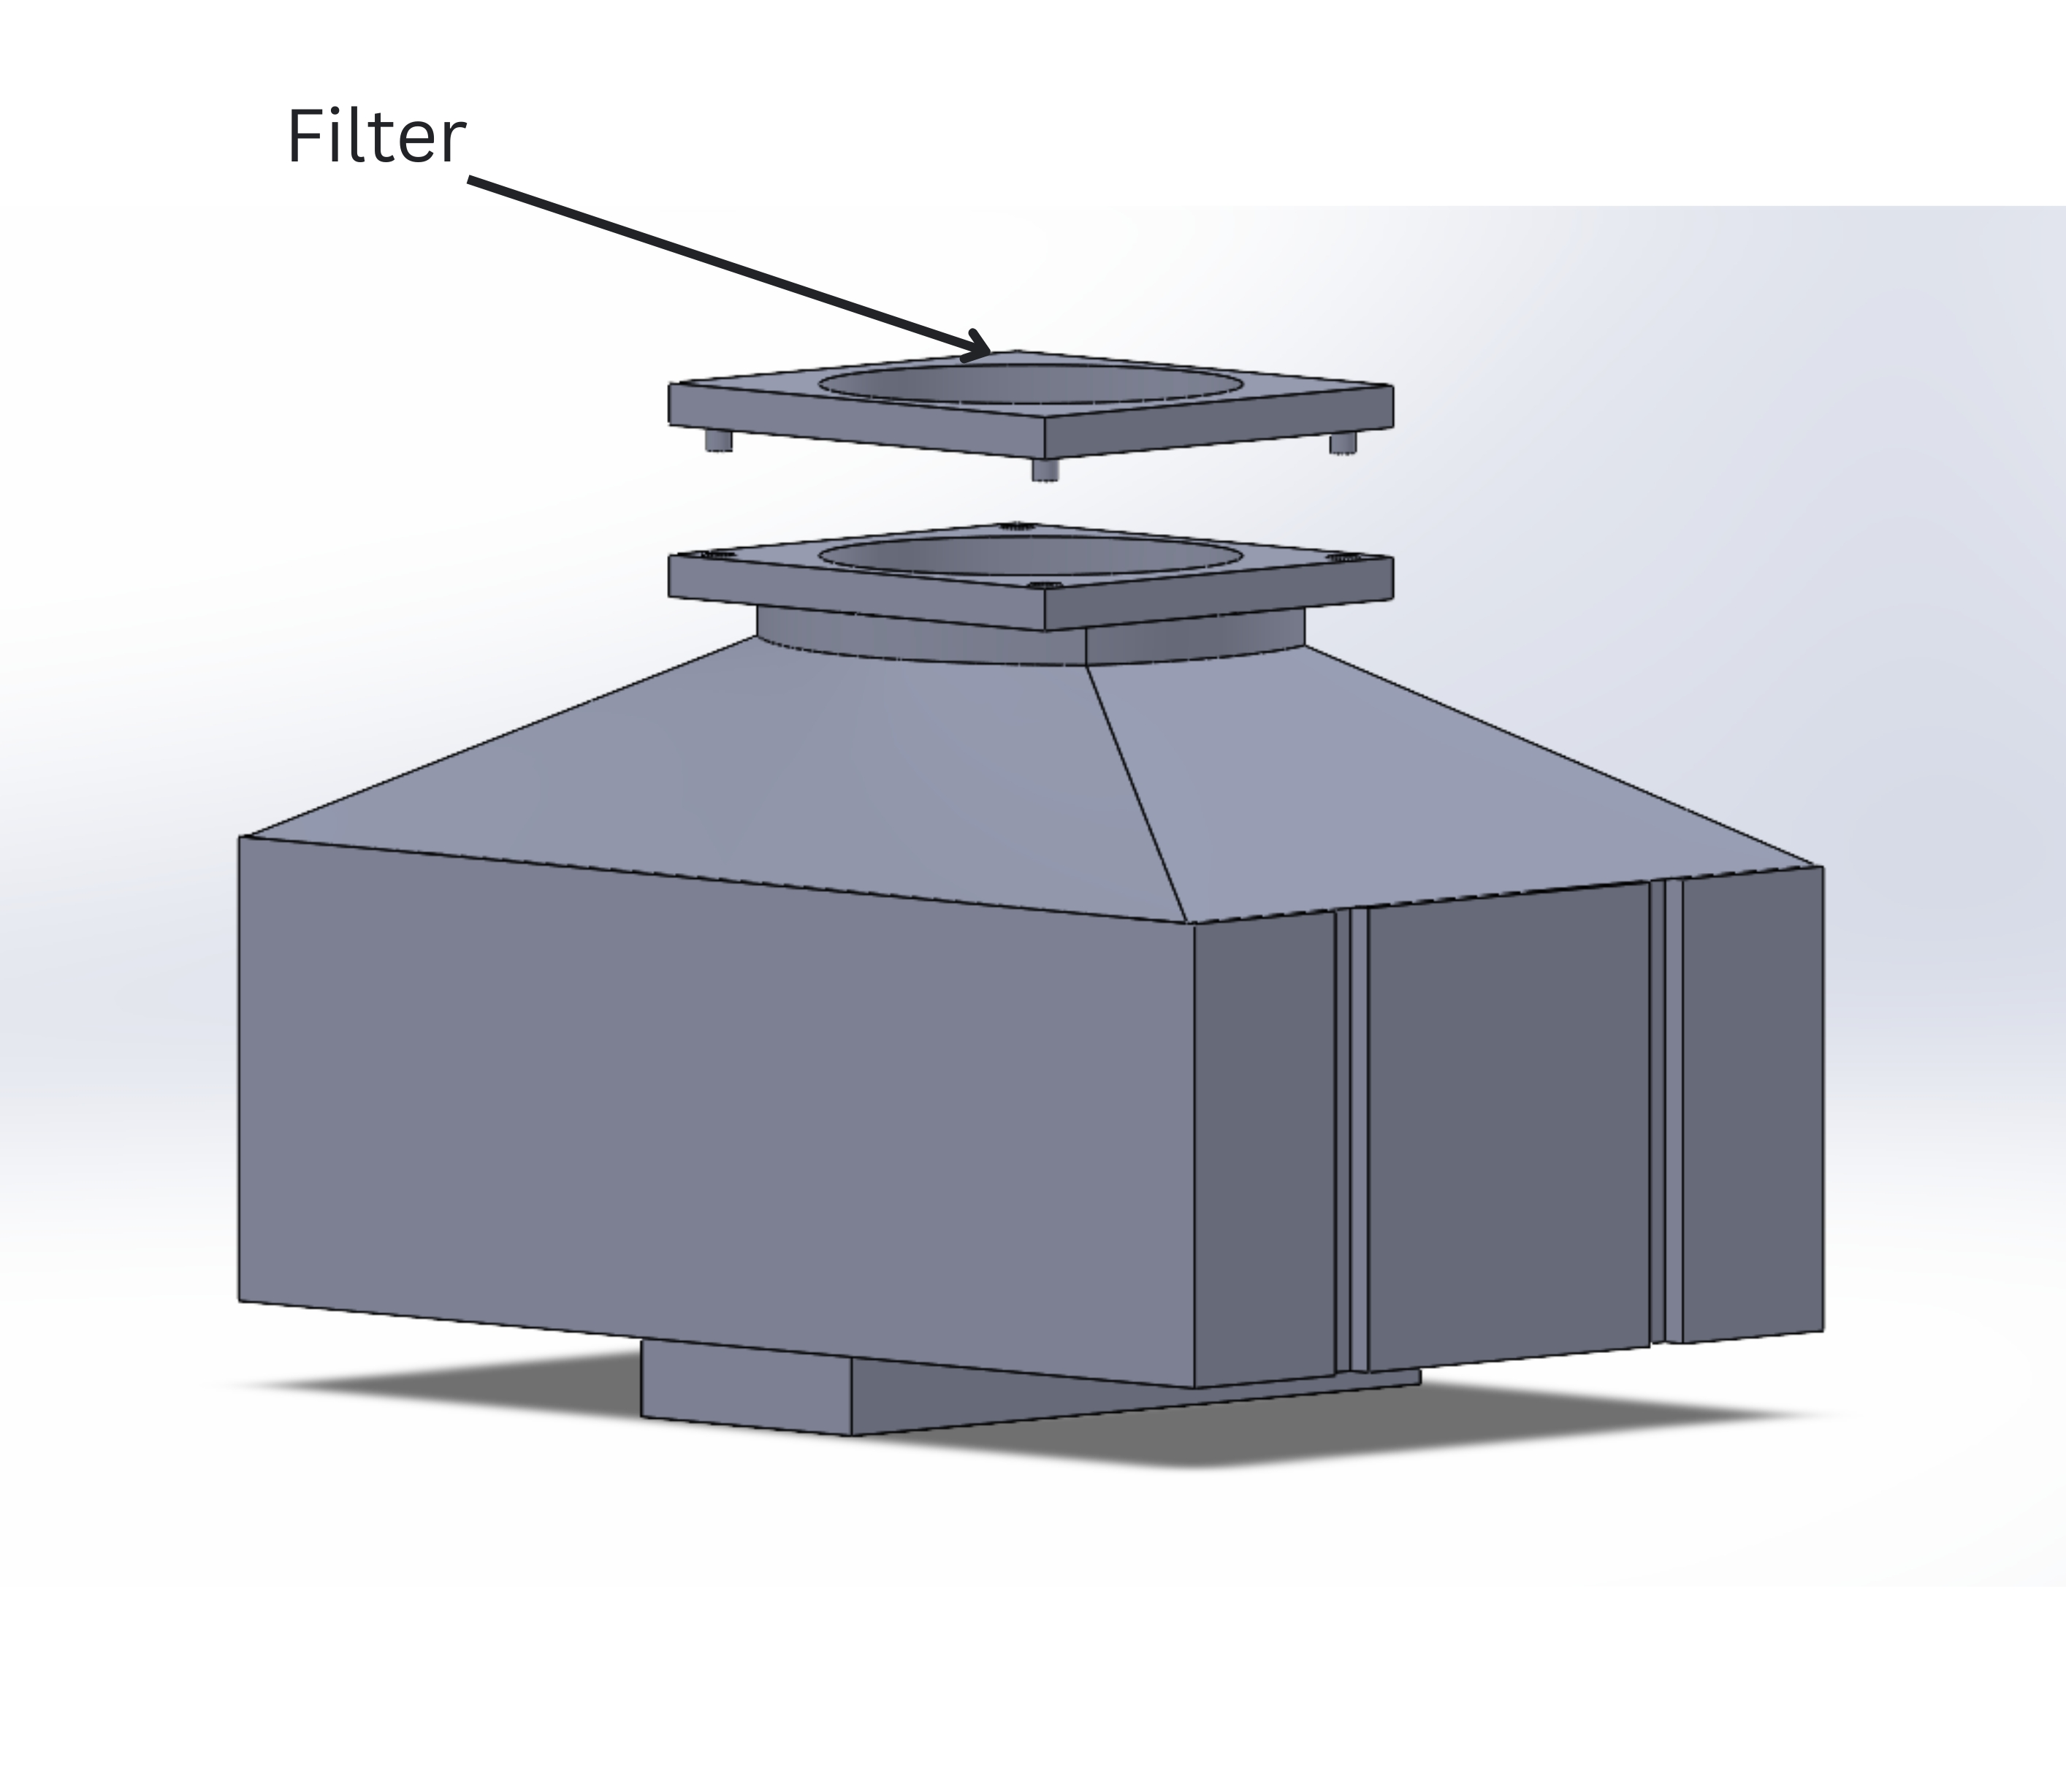
\includegraphics[width=1\textwidth, keepaspectratio]{images/cad/debris_chamber_cad.jpg}
    \caption{SolidWorks CAD design of the Debris Collection Chamber.}
    \label{fig:solidworks_debris_chamber}
\end{figure}
\begin{figure}[htbp]
    \centering
    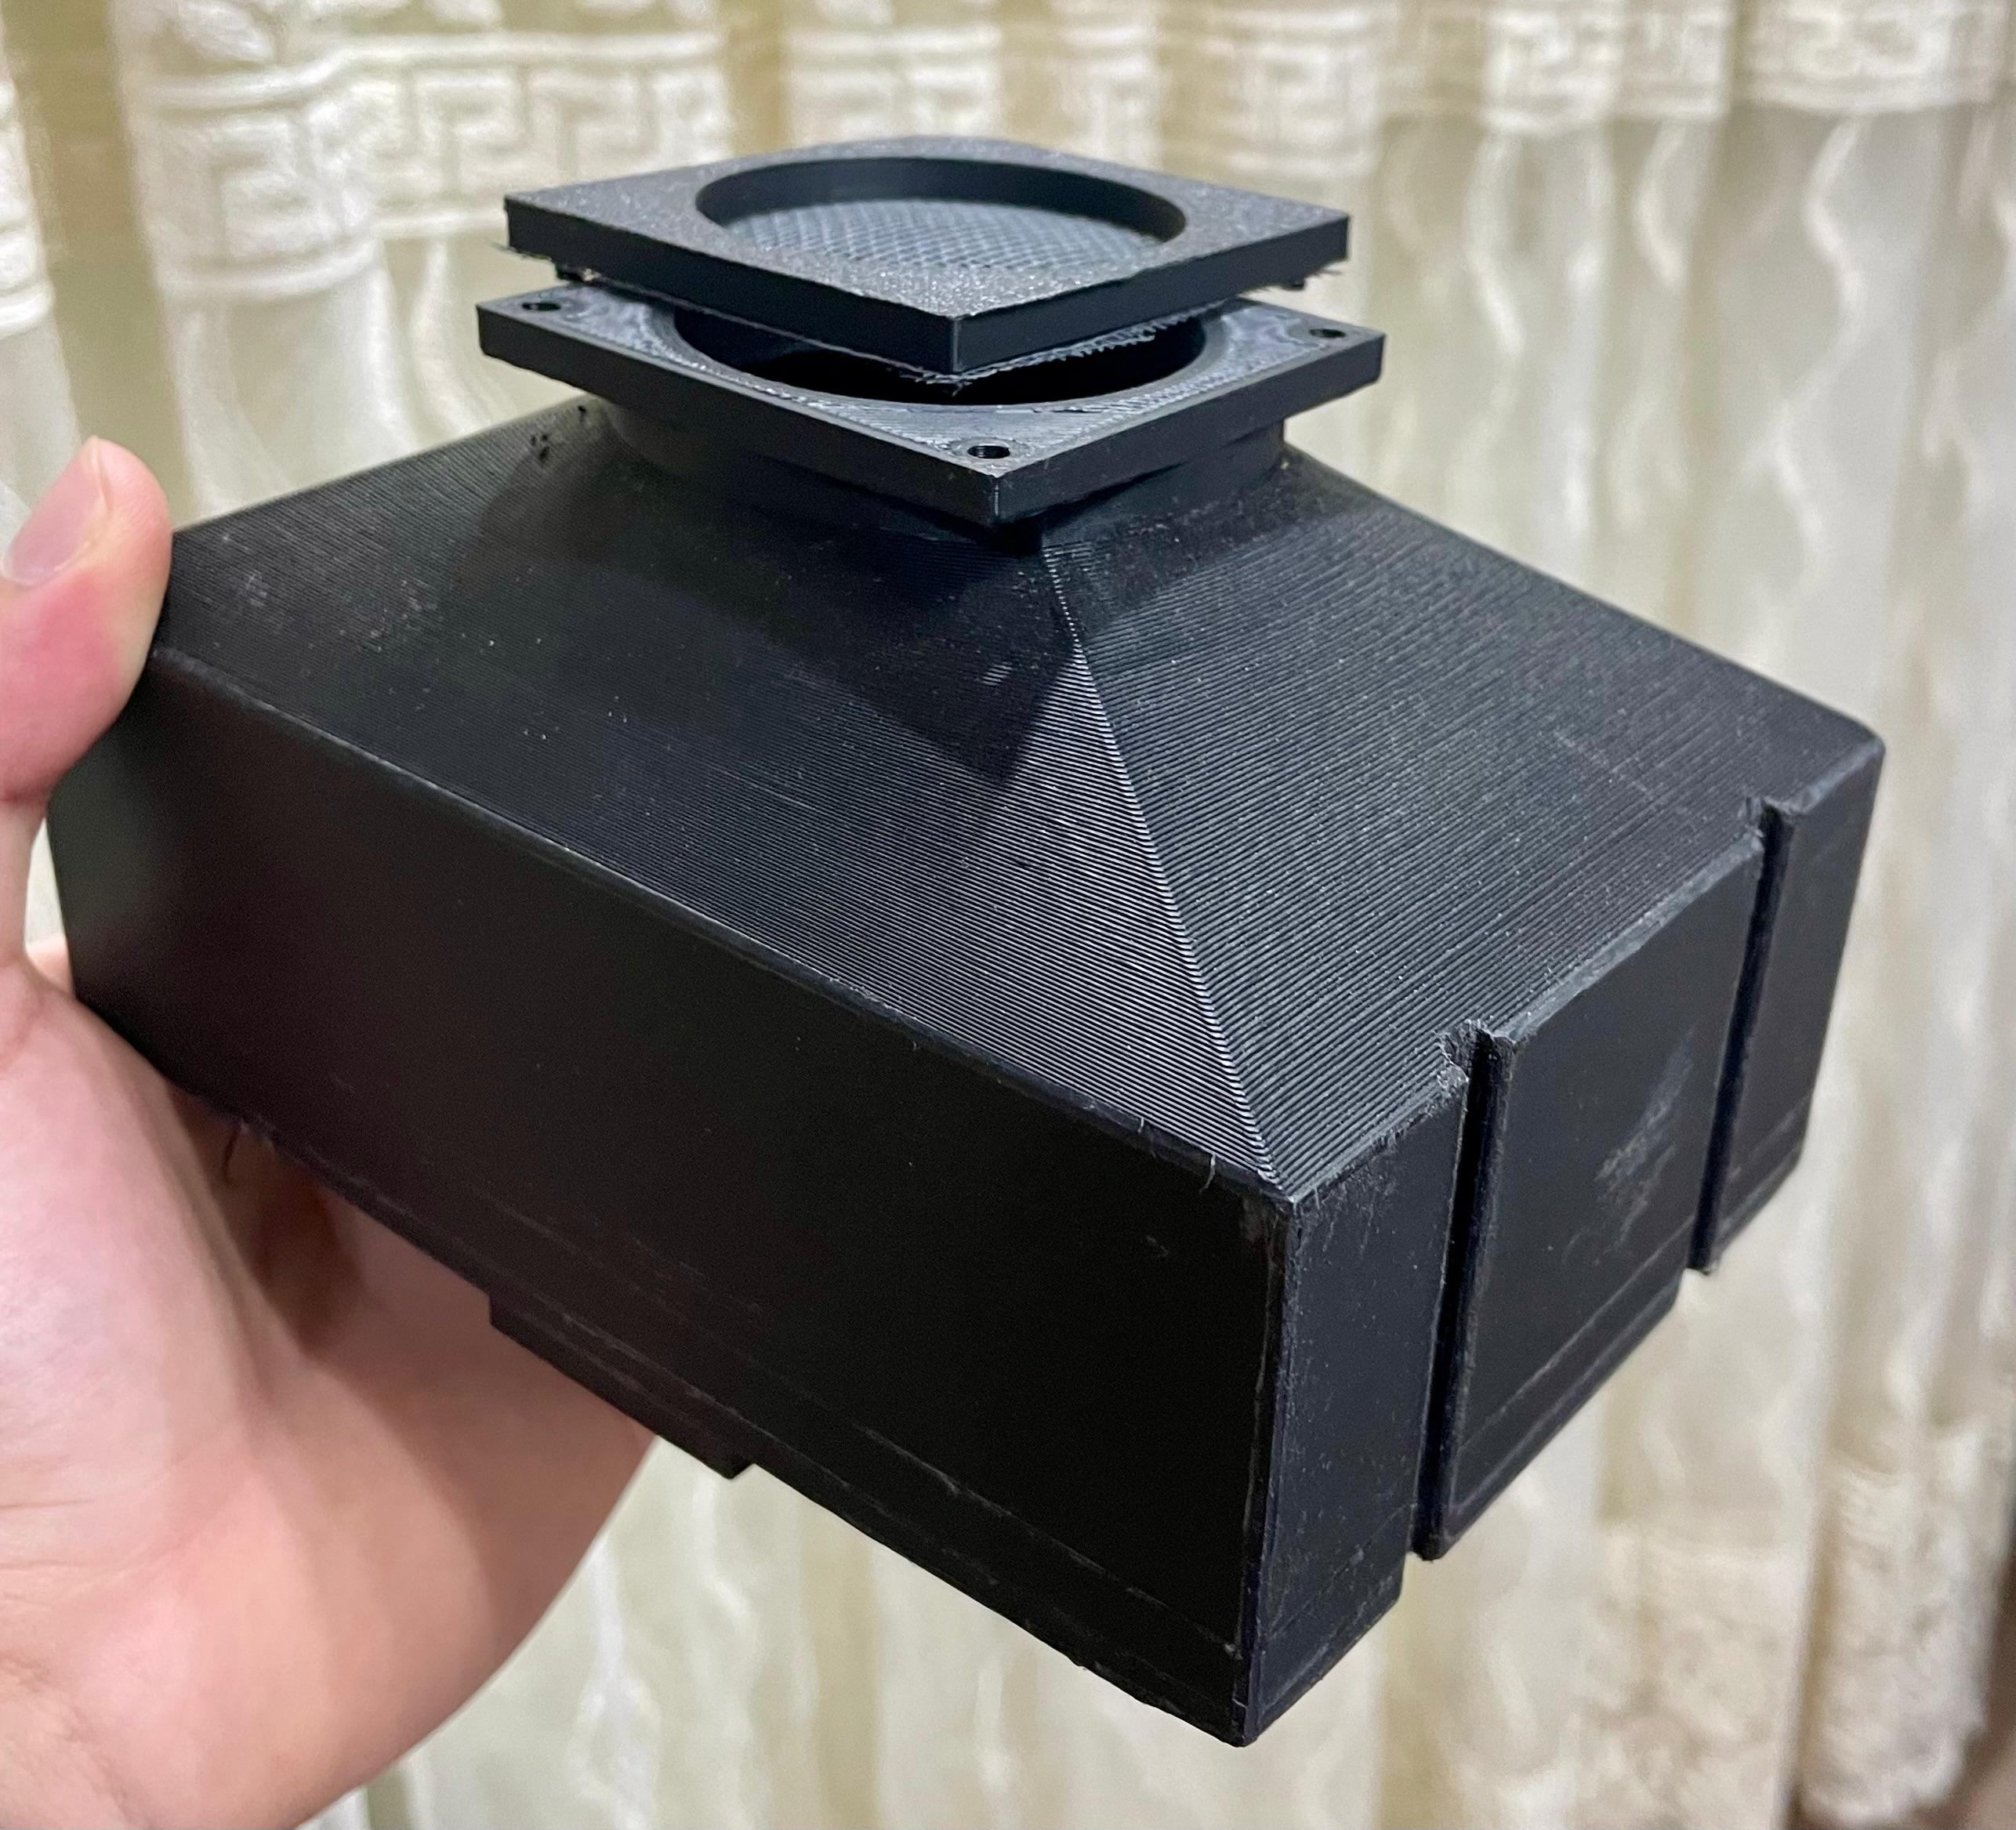
\includegraphics[width=0.75\textwidth, keepaspectratio]{images/photos/debris_chamber_photo.jpg}
    \caption{Photograph of the 3D printed Debris Collection Chamber with its removable filter lid.}
    \label{fig:debris_chamber_photo}
\end{figure}

The vacuum system is responsible for generating airflow to collect debris.
\begin{itemize}
    \item \textbf{Fan Selection and Mounting}: The primary vacuum source is a repurposed PS3 fan (Model: Delta KSB1012HE)~\cite{DeltaKSB1012HE_PSDevWiki}. This fan was readily available and met basic size and 12V \hyperref[term:dc]{DC} voltage requirements. It has a diameter of approximately 10cm and features 17 blades.
    The fan is mounted within the main top lid of the robot (see Figure~\ref{fig:sw_chassis_lid_iso}).
    \item \textbf{Airflow Path}: Air is drawn through an intake nozzle (part of the Debris Collection Chamber design, Figure~\ref{fig:solidworks_debris_chamber}), passes through the filter in the chamber's lid, then through the fan, and is exhausted from the robot. The debris chamber was designed to channel airflow with minimal obstruction.
\end{itemize}

\subsection{Drive System Design}
\label{subsec:drive_system_design_detailed}
The drive system enables the robot's mobility. A differential drive configuration was selected for its simplicity in control, maneuverability (allowing for zero-radius turns), and common availability of components.
\begin{itemize}
    \item \textbf{Motors and Wheels}: Two \hyperref[term:dc]{DC} gear motors (TT type) provide locomotion, each driving a 66mm diameter wheel. These are mounted in dedicated compartments at the rear of the chassis. (Visible in Figure~\ref{fig:sw_chassis_iso_open} and \ref{fig:sw_chassis_bottom_cad}).
    \item \textbf{Encoder Integration}: To enable precise movement control, a 20-slot plastic encoder disc was press-fit onto the interior side of each wheel's axle. An IR photoelectric sensor was mounted on the chassis such that the encoder disc passes through its 5mm groove. This setup allows for the measurement of wheel rotation, as detailed in Figure~\ref{fig:encoder_mechanism}.
    \item \textbf{Caster Wheel}: A caster wheel at the front provides a third point of contact, allowing for maneuverability and stable turns. As noted, the mounting of this wheel was adapted due to component availability. (Visible in Figure~\ref{fig:sw_chassis_bottom_cad} and Figure~\ref{fig:assembled_robot_bottom_photo}).
\end{itemize}

\begin{figure}[htbp]
    \centering
    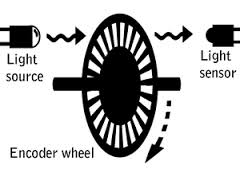
\includegraphics[width=0.47\textwidth]{images/components/encoder_disc_mounted.jpg}
    \caption{Diagram illustrating the principle of operation for the optical wheel encoder. As the encoder wheel (slotted disc) rotates with the main robot wheel, its slots alternately block and pass the light beam from the source to the sensor, generating a digital pulse train that corresponds to the distance traveled.}
    \label{fig:encoder_mechanism}
\end{figure}

\subsection{Main Robot Lid and Component Fastening}
\label{subsec:main_robot_lid_fastening_detailed}
The top lid of the robot (Figure~\ref{fig:sw_chassis_lid_iso}) serves multiple functions: it encloses the internal components, supports the vacuum fan assembly, presses down to secure the filter lid of the Debris Collection Chamber, and provides mounting points for an \hyperref[term:led]{LED} indicator and a power button. The main top lid incorporates dedicated openings for the power button and \hyperref[term:led]{LED} indicator, positioned conveniently next to the fan exhaust; these components are secured via friction fit. The method for securing the main top lid to the chassis was refined from an initial concept of small 3D-printed latching pieces to a more robust solution using four screws (detailed in Section~\ref{sec:mechanical_assembly_implementation_new}). The accessibility of the battery for charging was considered in the overall assembly.
\section{Mechanical Assembly Implementation}
\label{sec:mechanical_assembly_implementation_new}
The implementation process for the mechanical structure involved the fabrication of custom parts using an \hyperref[term:fdm]{FDM} 3D printer with \hyperref[term:pla]{PLA}+ filament (provided by a 3D printing service), and the assembly of all mechanical components onto the chassis.

The mechanical assembly followed a structured sequence:
\begin{enumerate}
    \item The two \hyperref[term:dc]{DC} gear motors and the front caster wheel were first secured to the 3D-printed chassis base.
    \item The custom 3D-printed Debris Collection Chamber was then slotted into its designated bay within the chassis.
    \item Electronic components, including the custom \hyperref[term:pcb]{PCB} (hosting the Raspberry Pi Pico W, LM2596S buck converter, and associated circuitry) and the \hyperref[term:l298n]{L298N} motor driver, were mounted onto their respective PCB spacers, which were affixed to the chassis. (The internal arrangement and wiring are detailed in Chapter~\ref{chap:electrical_control_performance}, Figure~\ref{fig:internal_wiring_photo_eval_new}).
    \item Essential wiring connections between the motors, sensors, \hyperref[term:pcb]{PCB}, and power components were then routed and made.
    \item The PS3 fan was installed into its housing within the main top lid.
    \item Finally, the top lid, with the fan, power button, and \hyperref[term:led]{LED} indicator secured, was fastened to the main chassis using four M3 screws, enclosing the internal components.
\end{enumerate}
An iterative design approach was crucial for refining certain mechanical aspects. For instance, the initial design for positioning the Debris Collection Chamber using slender guides proved too fragile. This was rectified by redesigning the mounting system to use two larger, screwed-in blocks with improved guide elements for precise placement and durability. Similarly, the main top lid fastening was changed from small latching pieces, found to be insufficiently robust against fan vibrations, to a more secure four-screw system. Minor adjustments, such as reaming mounting holes, were made as needed during assembly to ensure proper alignment and securement, a common practice in prototyping.

Figure~\ref{fig:assembled_robot_photos_eval_new} shows photographs of the fully 3D printed and assembled robot prototype. (The internal view showing component wiring and \hyperref[term:pcb]{PCB} integration is presented in Chapter~\ref{chap:electrical_control_performance}, Figure~\ref{fig:internal_wiring_photo_eval_new}).

\begin{figure}[htbp]
    \centering
    \begin{subfigure}[b]{0.496\textwidth}
        \centering
        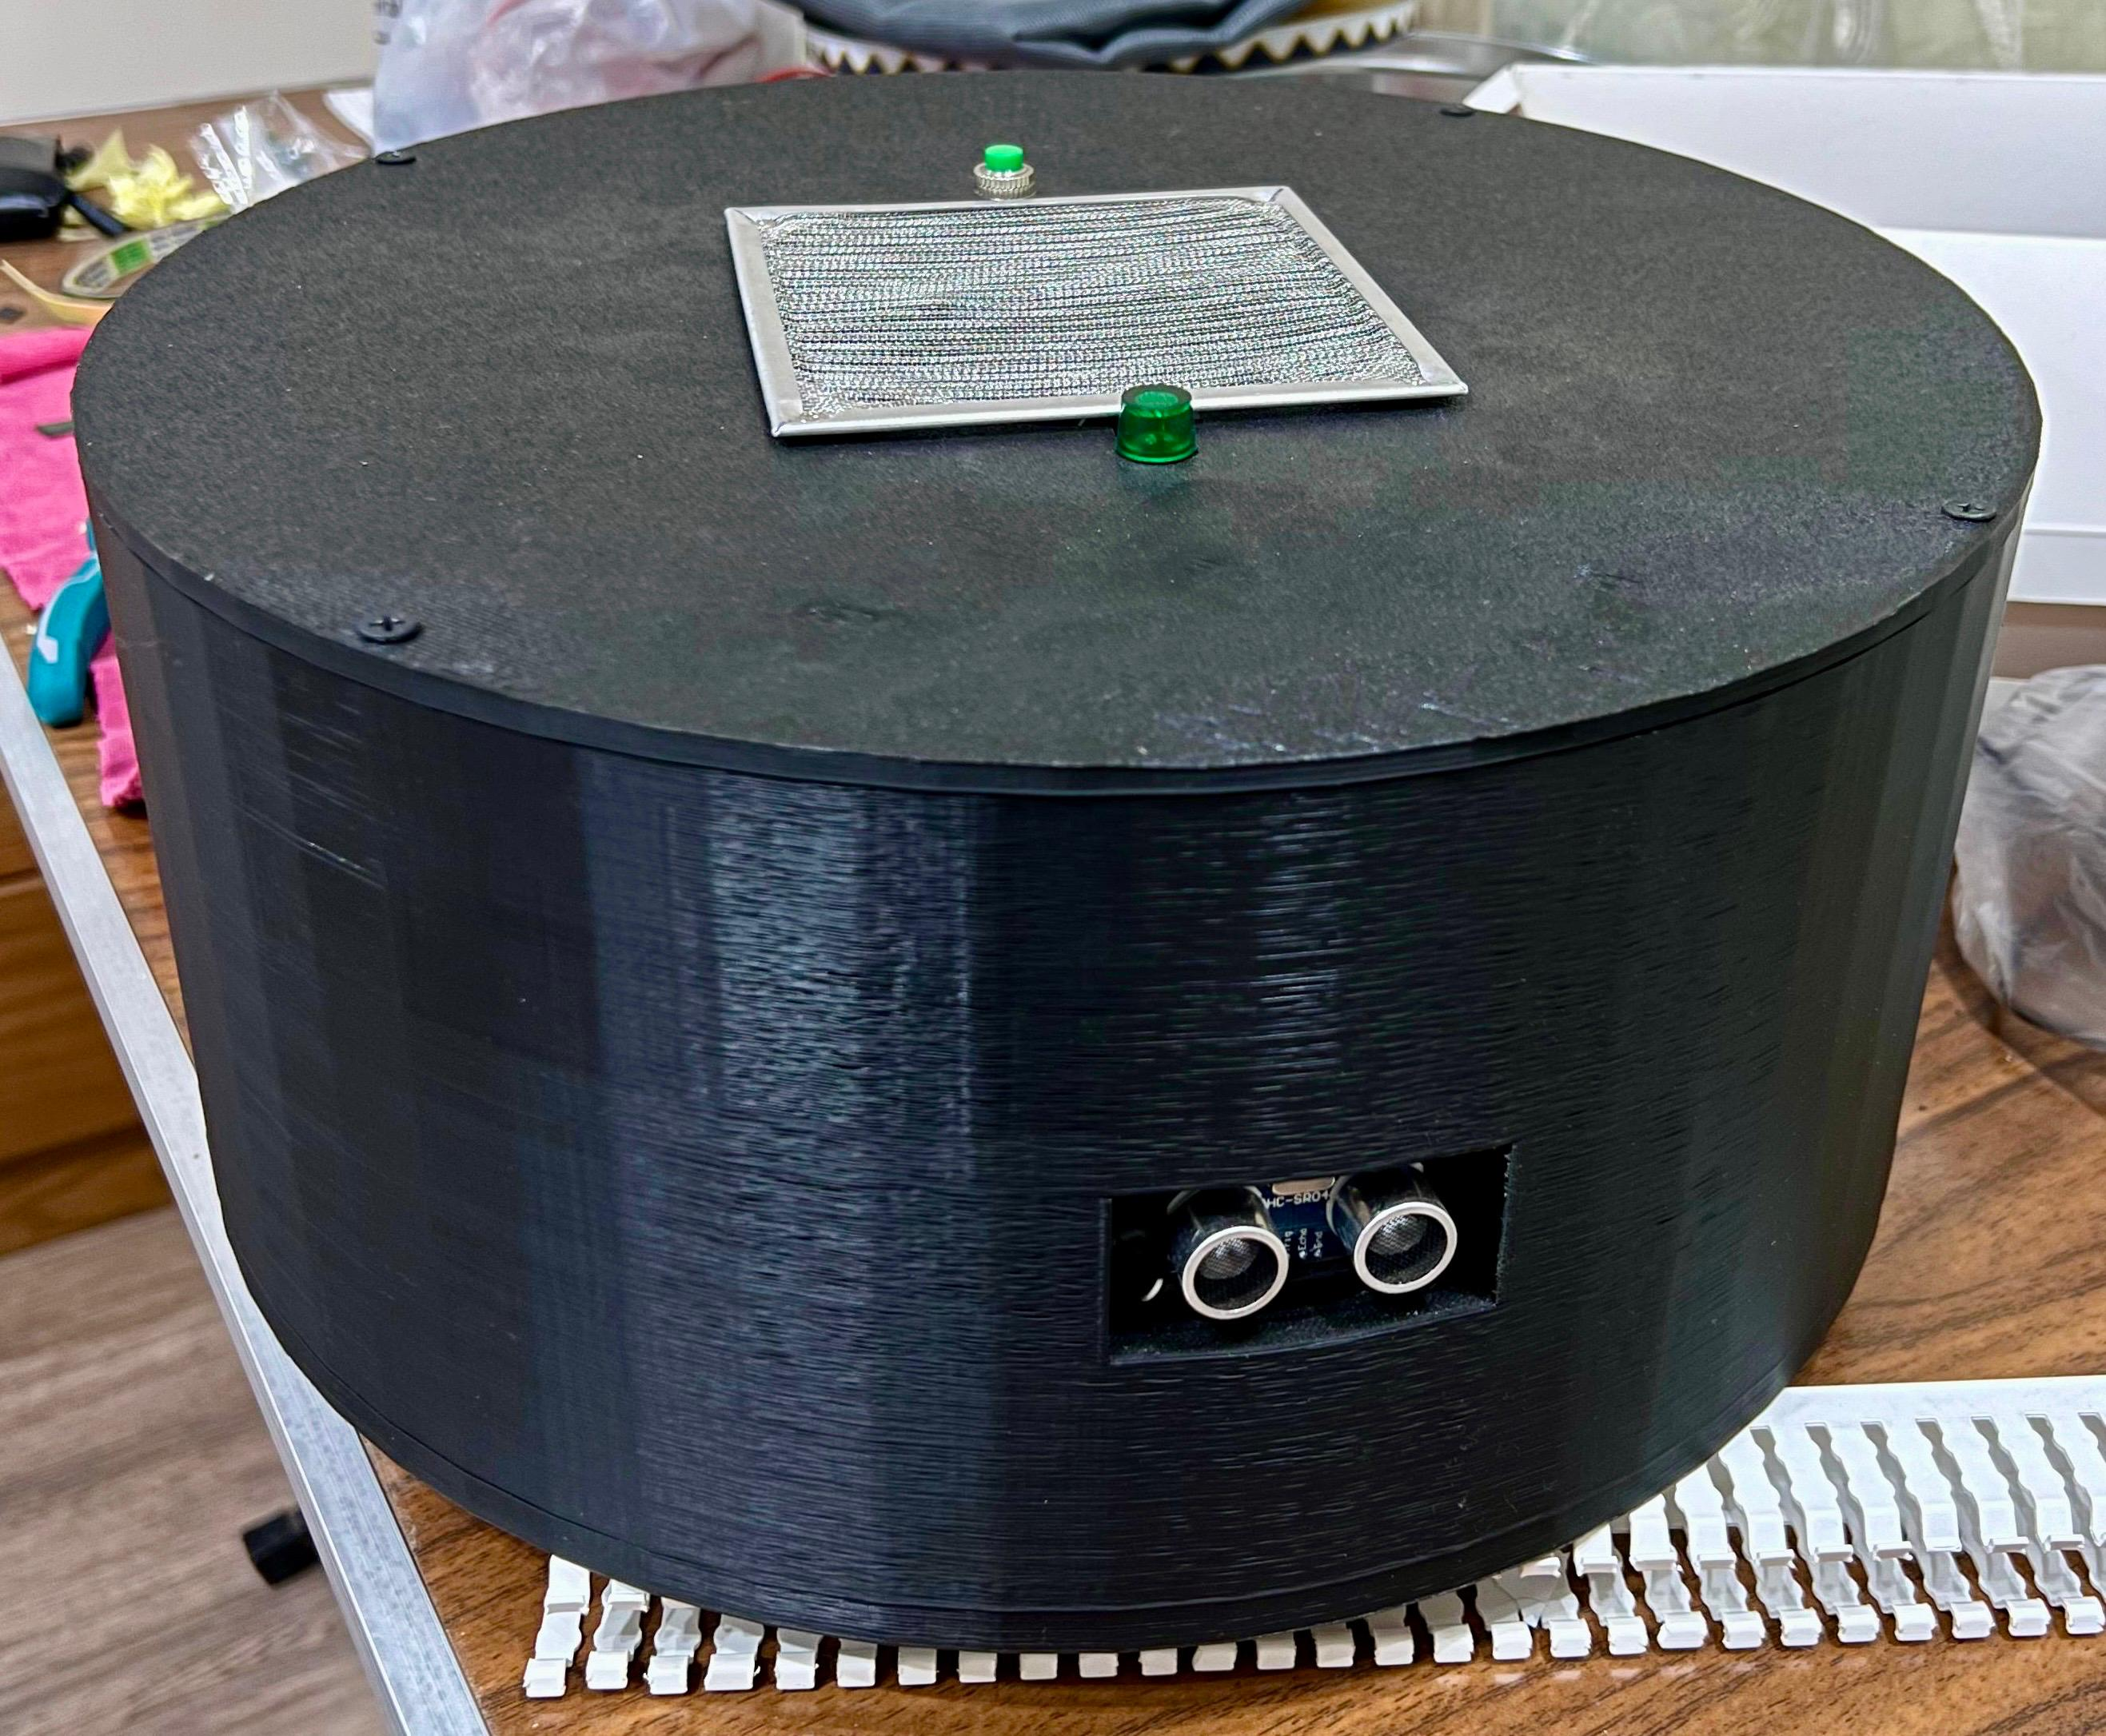
\includegraphics[width=\linewidth, keepaspectratio]{images/photos/robot_assembled_iso.jpg}
        \caption{Isometric view of the assembled robot.}
        \label{fig:assembled_robot_iso}
    \end{subfigure}
    \hfill % This adds some horizontal space between the images
    \begin{subfigure}[b]{0.496\textwidth}
        \centering
        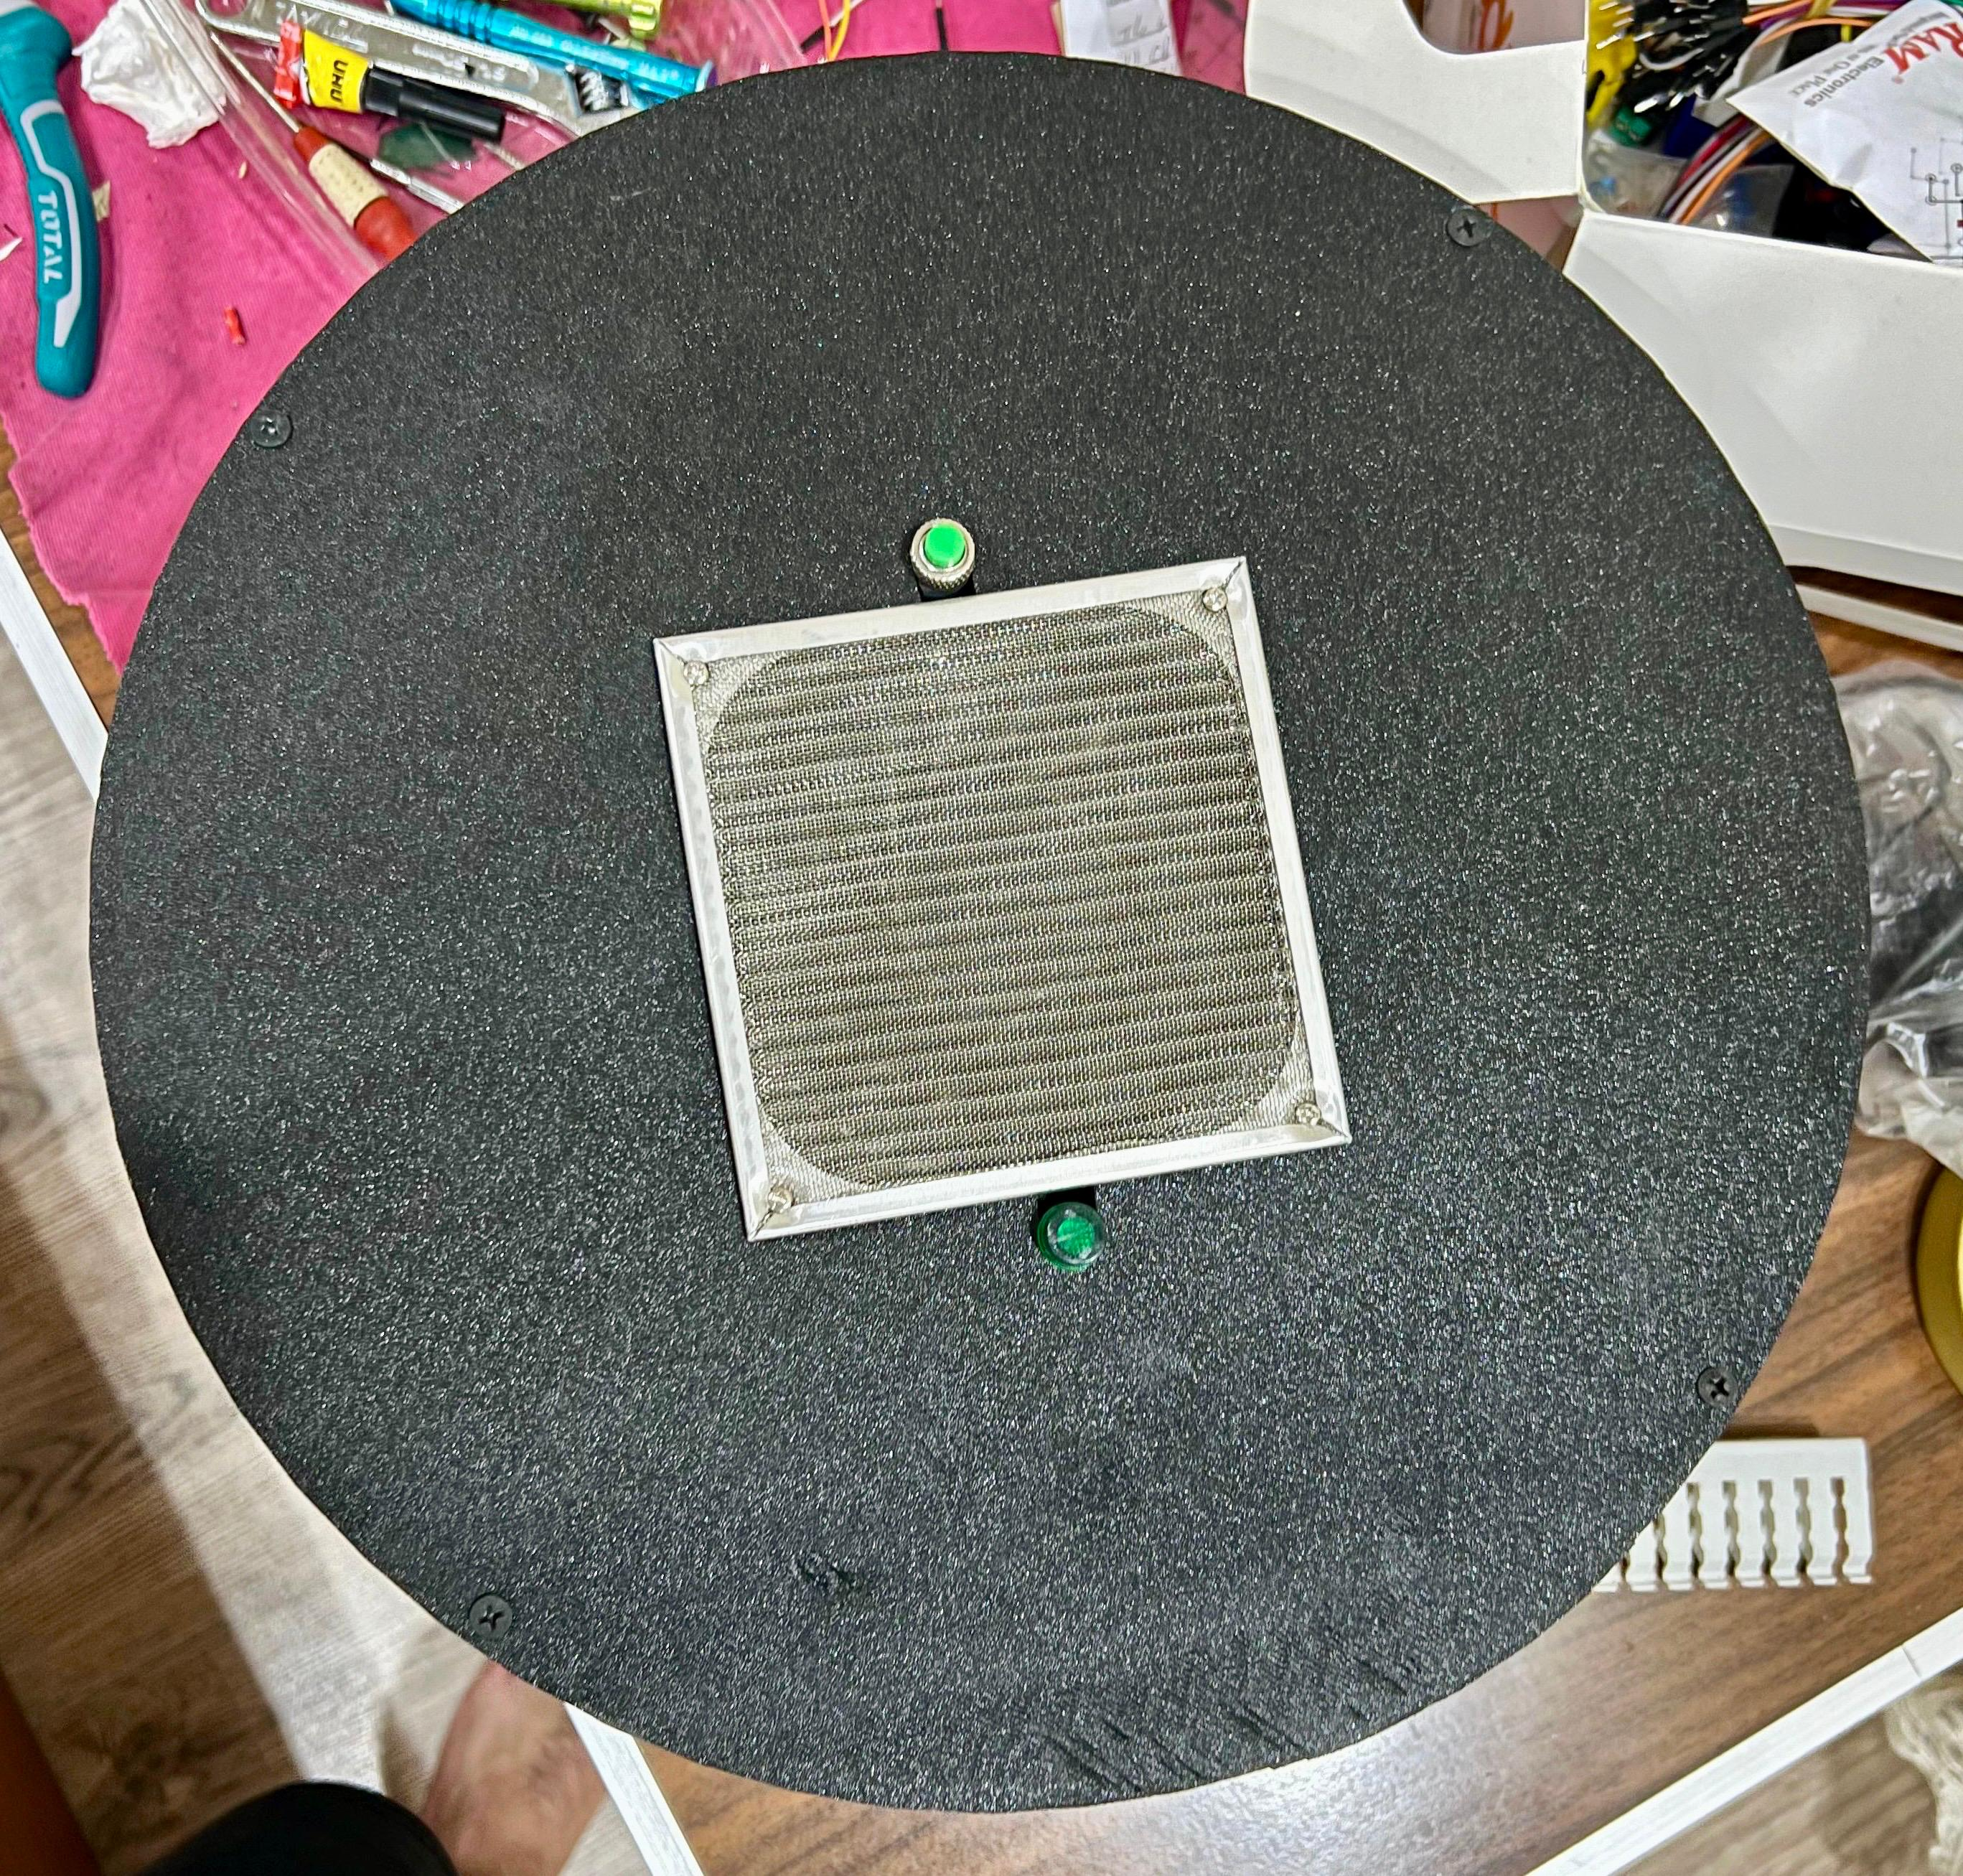
\includegraphics[width=\linewidth, keepaspectratio]{images/photos/robot_assembled_side.jpg}
        \caption{Top view of the assembled robot.}
        \label{fig:assembled_robot_side}
    \end{subfigure}
    \caption{Photographs of the 3D printed and assembled robot prototype.}
    \label{fig:assembled_robot_photos_eval_new}
\end{figure}